\graphicspath{{chapt_dutch/}{intro/}{simps/}}

% Header
\renewcommand\evenpagerightmark{{\scshape\small Chapter 5}}
\renewcommand\oddpageleftmark{{\scshape\small Media Grids}}

\renewcommand{\bibname}{References}

\hyphenation{}

\chapter{Search for SIMPs using Trackless Jets}
\label{ch:SIMPs}

\section{Introduction}

\section{Trigger Selection}


The following appendix describes the studies that have been done for the analysis and explains the reasons that a single jet trigger has been selected. Several triggers have been designed specifically for this analysis. These are summarized in Table~\ref{tab:triggers}. Four signal triggers are available, providing a trade off between as high ChF cut and as low jet $p_T$ cut. The ChF cut is always applied on both jets.


\begin{table}[h]
  \centering
  \begin{tabular}{| l | c | c | c |}
    \hline
    Trigger name & Type & Run range & Int. Lumi. \\
    \hline
    \verb|HLT_DiCentralPFJet170_CFMax0p1_v*|     & Signal  & $> 274748$      & $33.1 \, \mathrm{fb}^{-1}$ \\
    \verb|HLT_DiCentralPFJet220_CFMax0p3_v*|     & Signal  & $274748-281084$ & $5.91 \, \mathrm{fb}^{-1}$ \\
    \verb|HLT_DiCentralPFJet330_CFMax0p5_v*|     & Signal  & $> 274748$      & $33.1 \, \mathrm{fb}^{-1}$ \\
    \verb|HLT_DiCentralPFJet430_v*|              & Signal  & $> 274748$      & $33.1 \, \mathrm{fb}^{-1}$ \\
    \verb|HLT_DiCentralPFJet170_v*|              & Control & $> 274748$      & $0.101 \, \mathrm{fb}^{-1}$ \\
    \verb|HLT_SingleCentralPFJet170_CFMax0p1_v*| & Control & $> 274748$      & $0.375 \, \mathrm{fb}^{-1}$ \\
    \hline
  \end{tabular}
  \caption{Summary of the triggers used for this analysis.}
  \label{tab:triggers}
\end{table}


These trigger paths were designed by using QCD samples to test their performance before using them in data-taking, since the signal samples do not simulate the trigger behavior. The trigger efficiency of $HLT\_DiCentralPFJet330\_CFMax0p5$ as a function of $p_{T}$ and ChF is shown in Figure~\ref{fig:efficiencies_qcd_data}, data in black and QCD in red. After further discussions and investigation it was understood that QCD cannot emulate adequately the signal behavior at very low ChF. A proposed solution was to measure the efficiency by taking a $\gamma+$jet sample, match the photon to the leading jet and measure the efficiency at low ChF. The problem with this method was that the photon in many cases is reconstructed as an electron by the PF algorithm. Thus, the jet is reconstructed with large EMF and it does not mimic our signal. 

The solution to the signal-like simulation was given by generating a dineutron sample, using the kinematics of the SIMP sample with mass $m_{\chi}=700$~GeV. This was achived by replacing the particle ID of SIMPs with neutrons in the LHE files and run the full simulation. Figure~\ref{fig:efficiencies_simp_data} shows the trigger efficiency of $HLT\_DiCentralPFJet330\_CFMax0p5$ as a function of $p_{T}$ and ChF, data in black and signal-like MC in red. After investigating the HLT code it was found that a filter ($HLTPFJetIDProducer$) in the paths requires at least one charged particle in the jets. This explains why the trigger efficiencies turn on at the expected values when using data or QCD while it is largely inefficient in signal-like simulation.




\begin{figure}[h]
  \centering
  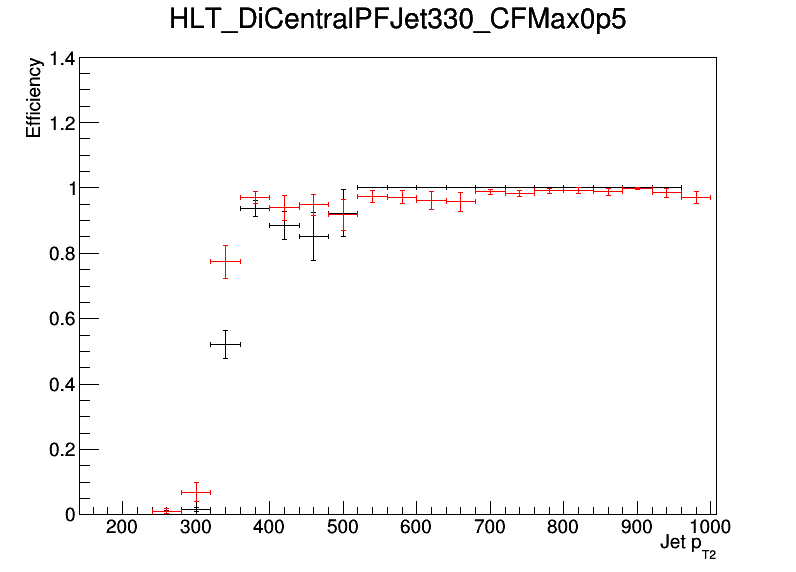
\includegraphics[width=0.5\textwidth]{figures/trigger/pt_eff_05_DataMC.png}\hfill%
  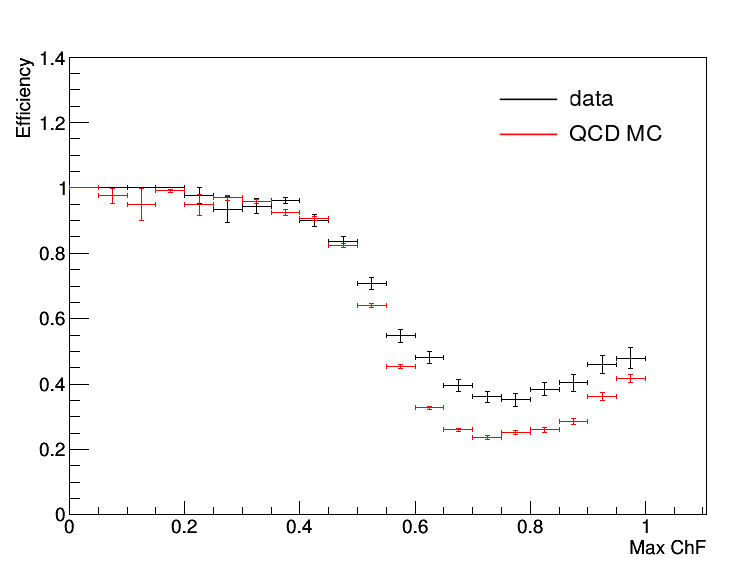
\includegraphics[width=0.5\textwidth]{figures/trigger/chf_eff_05_DataMC.png}
  \caption{Trigger efficiency as a function of $p_{T}$ (left) and ChF(right). Comparison between data(black) and QCD(red). }
  \label{fig:efficiencies_qcd_data}
\end{figure}


\begin{figure}[h]
  \centering
  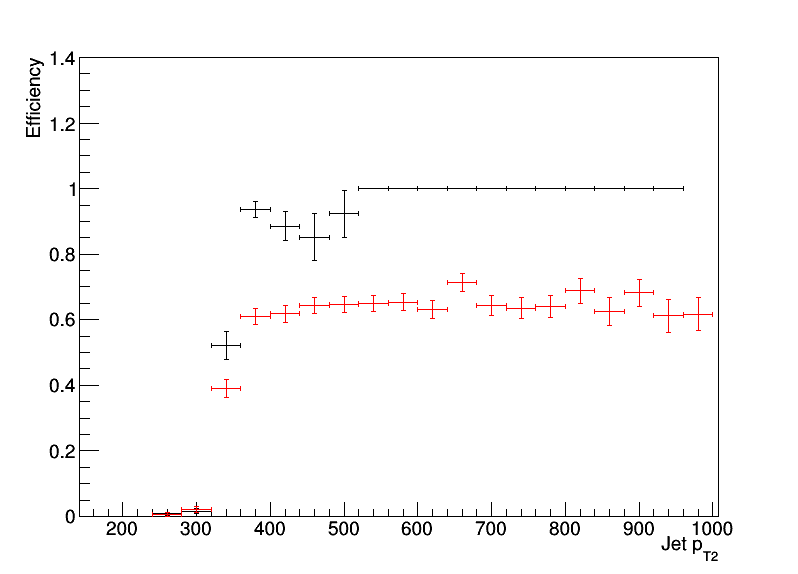
\includegraphics[width=0.5\textwidth]{figures/trigger/pt_eff_05_DataSIMP.png}\hfill%
  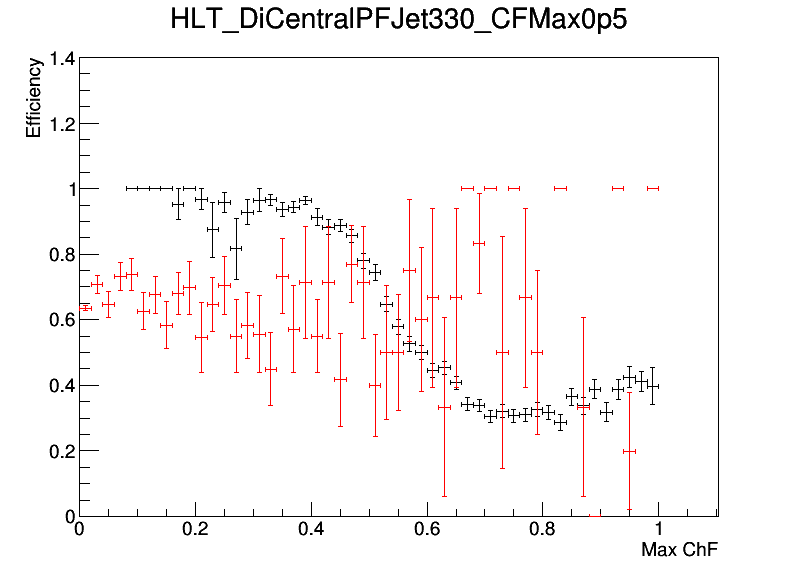
\includegraphics[width=0.5\textwidth]{figures/trigger/chf_eff_05_DataSIMP.png}
  \caption{Trigger efficiency as a function of $p_{T}$ (left) and ChF(right). Comparison between data(black) and signal-like MC(red).}
  \label{fig:efficiencies_simp_data}
\end{figure}

The single jet trigger \texttt{HLT\_PFJet450} has been used for the analysis. The trigger was selected since it has the lowest threshold among the unprescaled single jet triggers. Appendix~\ref{sec:aptrigger} describes the studies that led to the selection of the particular HLT trigger. 

The trigger efficiency for the data was measured using the SingleMuon dataset. It is defined as:

\begin{equation}
\epsilon_{Y} = \frac{\mathrm{Obs}(\texttt{HLT\_Jet450}\ \mathrm{and}\ \texttt{HLT\_IsoMu24})}{\mathrm{Obs}(\texttt{HLT\_IsoMu24})}
\end{equation} 

where Obs in this case is the $p_T$ spectrum of the leading jet for events that fired the single muon (and single jet) trigger. The jets are required to have muon fraction less than $0.3$ in order to avoid jets with large difference in the online and offline $p_T$. This can happen if the particle flow jet contains a high $p_T$ muon that can significantly change the total $p_T$ of the jet between online and PF jet, given that the online jet is reconstructed using information only from the calorimeters.

The efficiency was also measured in the QCD and a signal-like sample. In this case the denominator is the $p_T$ spectrum of leading jet without any trigger selection while the numerator the spectrum with the requirement to fire the single jet trigger. For the signal-like sample a dineutron sample was used, using the kinematics of the SIMP sample with mass $m_{\chi}=\SI{700}{GeV}$. This was achieved by replacing the particle ID of SIMPs with neutrons in the LHE files and run the full simulation.

Figure~\ref{fig:ptturnon} shows the turn on curves for data (black), QCD (red), and signal-like MC (blue). The trigger efficiency was found to be $98\%$ for jets with $p_{T}>550$ GeV (green dashed line).

\begin{figure}[h]
  \centering
  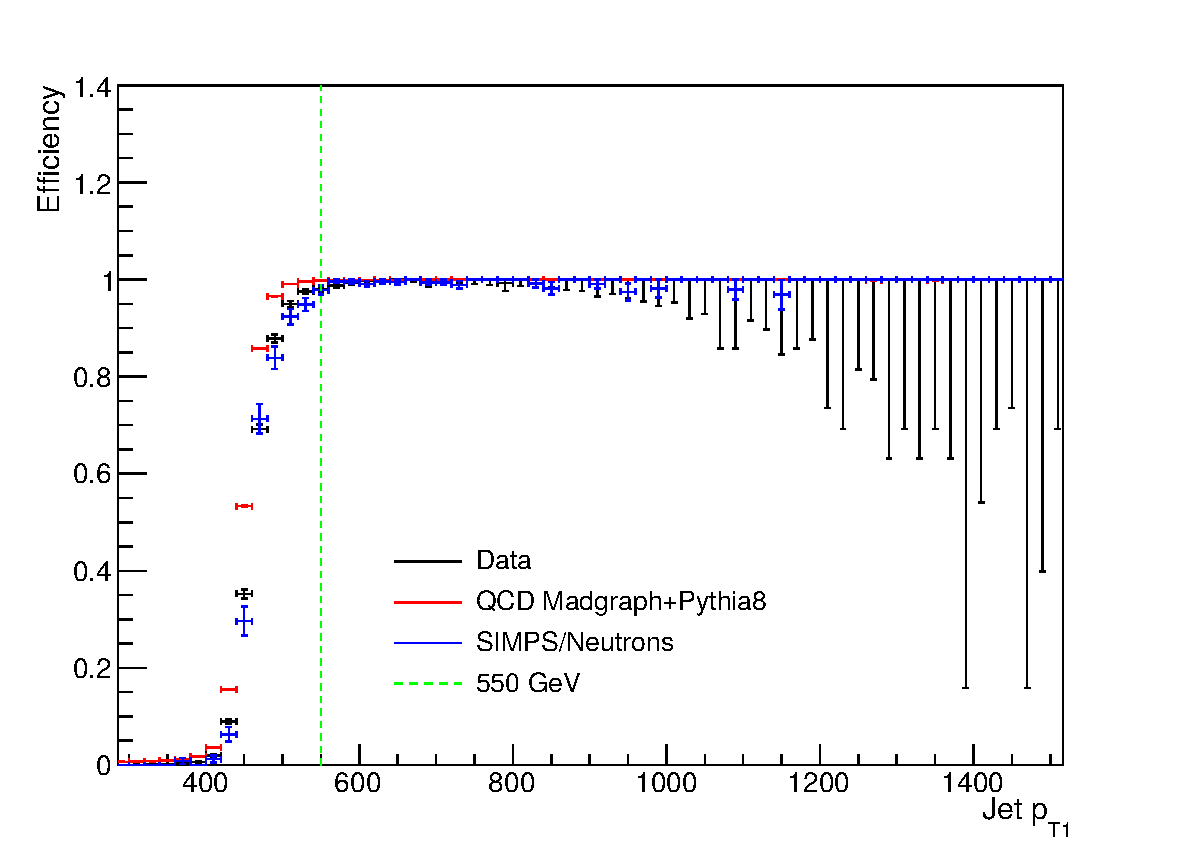
\includegraphics[width=0.6\textwidth]{figures/trigger/pt_HLT_PFJet450.pdf}
  \caption{Trigger efficiency turnon as a function of the offline leading jet $p_T$.}
  \label{fig:ptturnon}
\end{figure}

\section{Event selection}

The event selection aims to select back-to-back dijet events with a low ChF. As a baseline selection, we select the two highest-$p_T$ jets to have $p_T > \SI{550}{GeV}$, to ensure the jets to be above the turnon of the trigger. Furthermore, we require for these jets $|\eta| < 2.0$, placing these jets fully within the tracking volume, thus suppressing backgrounds from jets that have a low ChF due to tracks falling out of tracker acceptance. 
%The azimuthal separation of the two selected jets is then required to be $\Delta\phi > 2$. 

Since SIMPs do not undergo parton shower, while QCD partons undergo final state radiation, events with SIMPs have a lower number of jets than QCD multijet events (see Figure~\ref{fig:event_selection_2}, top right). We therefore require that, apart from the two leading jets, no additional jets in the event are found with $p_T>\SI{30}{GeV}$ in the full $\eta$ acceptance of the CMS calorimeters. 
%This requirement already selects out back-to-back jets and an additional cut on the azimuthal separation between the jets was indeed found not to impact signal-background separation.

We also apply a photon veto to suppress $\gamma$+jets events. This is done by rejecting events with a photon within $\Delta R < 0.1$ of the leading or subleading jet, using the loose working point (WP) of the cut based photon ID to identify photons, as described before. In some cases, though, jets have a large photon energy fraction (larger than $0.8$) but the photon in the jet does not pass the loose ID cuts. These are for instance cases where there is a photon conversion in the tracker and as a result the photon fails to pass the loose ID cuts. In these cases that the photon in the jet does not pass the loose WP and the photon energy fraction of the jet is greater than $0.8$, an additional cut is applied. The jet, and as a result the event, is rejected if conversions with $p_{T,conv} / p_{T,\gamma} > 0.3$ are matched to the photon within $\Delta R < 0.2$. Additionally, the 2 jets are required to have a neutral electromagnetic energy fraction lower than 0.9, corresponding to one of the standard tight jet ID requirements. We do not apply the full jet ID, since the requirements on e.g. the neutral hadronic energy fraction and the charged multiplicicty would reject the signal.

We require there to be at least two reconstructed vertices in the events, to avoid any problems related to the striking data/MC discrepancy we observe for events with only one reconstructed vertex (see  Figure~\ref{fig:event_selection_2}, top left). The azimuthal separation of the two selected jets is required to be $\Delta\phi > 2$. Finally, the recommended MET filters are applied~\cite{filters}.

Table~\ref{tab:cutflow} shows the number of events remaining in data and for 2 signal samples, after consecutively applying the described selection cuts. In Figure~\ref{fig:event_selection}, we show after these selections the comparison between data, QCD multijet simulation, and signal, for the $$p_T$$, $\eta$ and ChF of the two leading jets. Figure~\ref{fig:event_selection_2} shows the number of vertices, number of jets, $\Delta\phi(\mathrm{jet}1, \mathrm{jet}2)$, and the $H_{T}$ of the events. In some cases, we removed the cut of the variable being shown. The bump and long tail that can be seen in the data for the $\Delta\phi(\mathrm{jet}1, \mathrm{jet}2)$ distribution contain events coming from processes with a heavy vector boson, such as Z + jets or W + jets, or $t\bar{t}$ events. The MC instead shows a steeply falling spectrum since only QCD dijet events are shown.

\renewcommand{\arraystretch}{1.4}
\begin{table}[h]
  \centering
\begin{tabular}{| l | r | r | r | r |}
\hline
\multirow{2}{*}{selection cut} & \multicolumn{4}{ c |}{yield}\\
\cline{2-5}
 & \multicolumn{1}{c|}{data} & \multicolumn{1}{c|}{QCD MC} & SIMP ($m_{\chi} = 1$ GeV) & SIMP ($m_{\chi} = 1000$ GeV) \\
 \hline
$p_T^{j1, j2}>550$ GeV & 2540420 & 3152550 & 773 & 5.7 \\
$|\eta_{j1, j2}|<2.0$ & 2441240 & 2980320 & 748 & 5.6 \\
\# jets = 2 & 534053 & 587670 & 636 & 4.9 \\
photon veto & 531366 & 586674 & 636 & 4.9 \\
\# vertices $\geq$ 2 & 531244 & 586641 & 636 & 4.9 \\
 $\Delta\phi(j1, j2) > 2$ & 531207 & 586641 & 636 & 4.9 \\
MET filters & 528614 & 582184 & 634 & 4.9 \\
\hline
\end{tabular}
\caption{Number of events remaining after the listed selection cuts in data, and for 2 signal samples as well.}
\label{tab:cutflow}
\end{table}

\begin{figure}[h!]
  \centering
  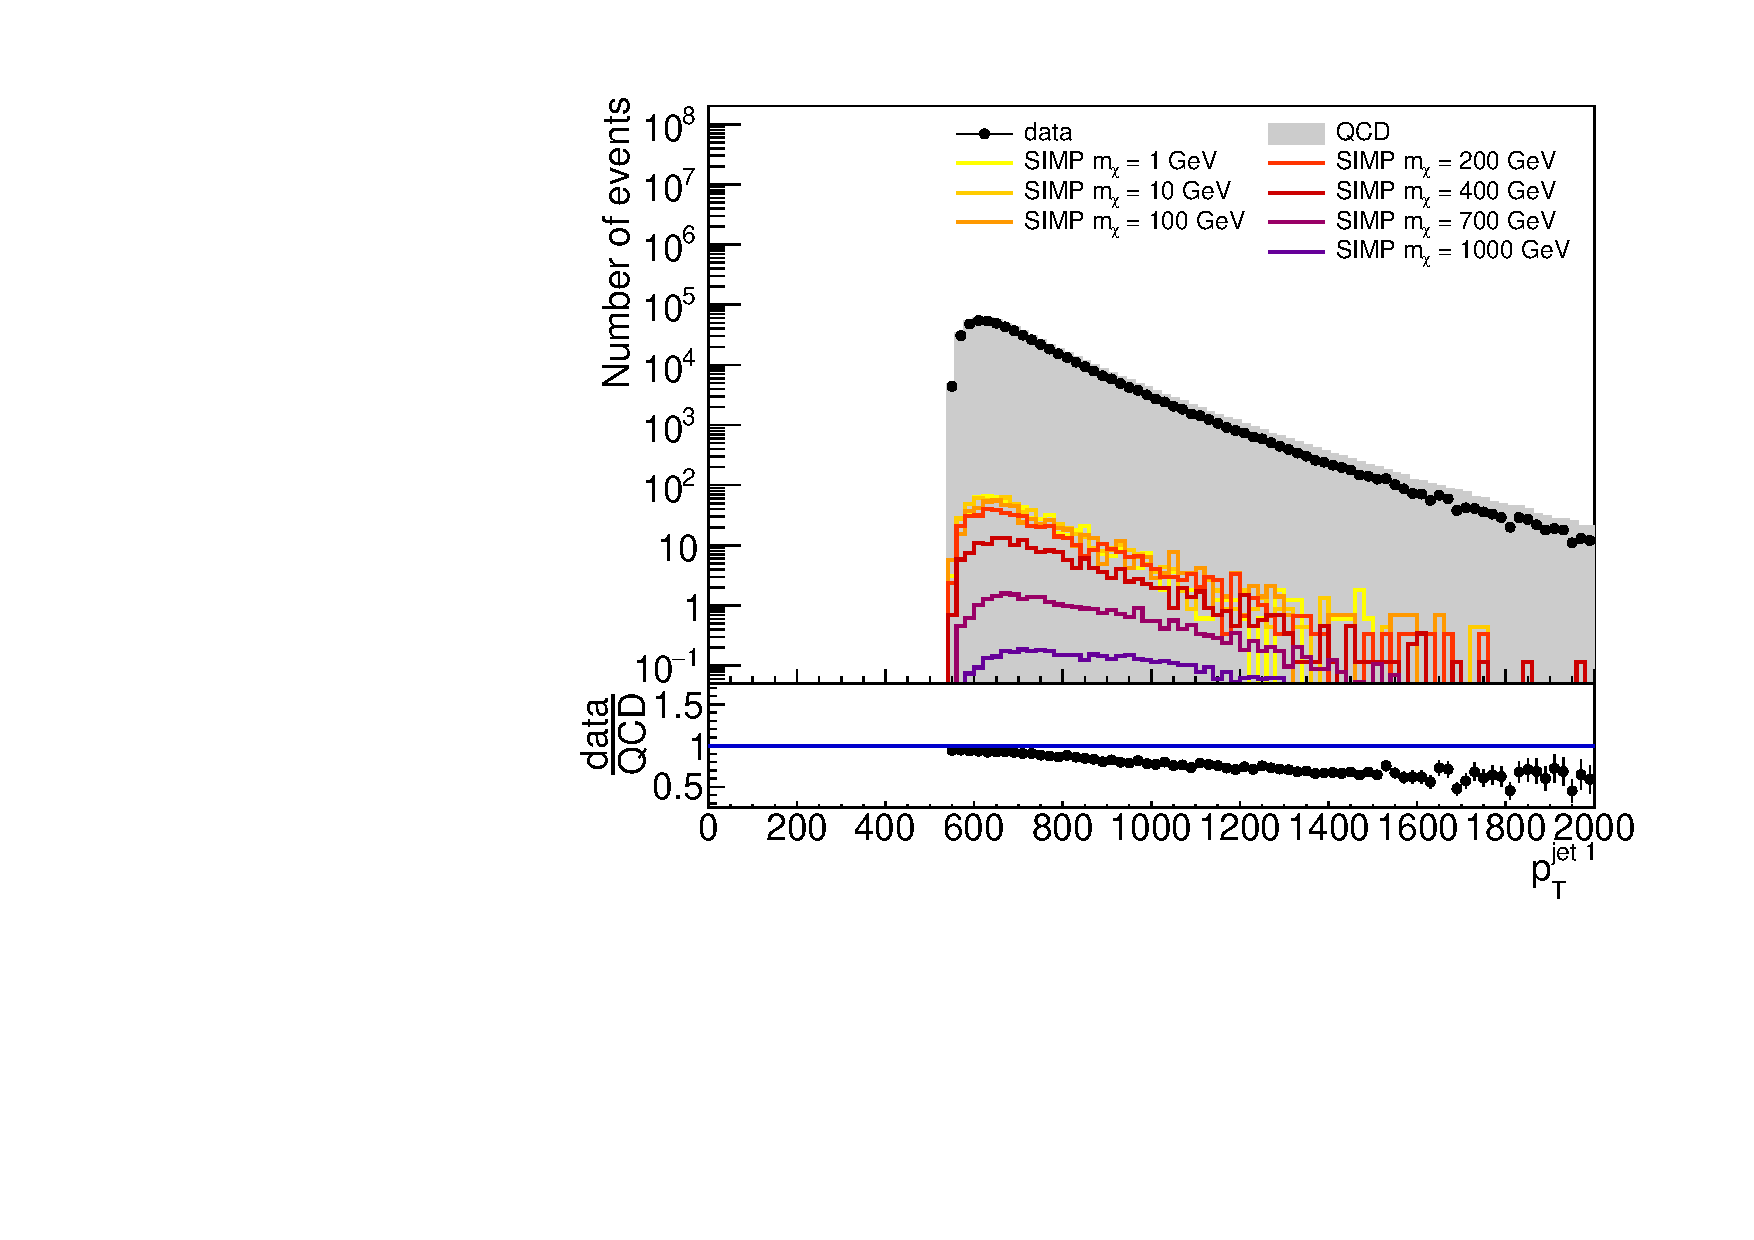
\includegraphics[width=0.5\textwidth]{figures/jet1_pt_newtrigger}\hfill%
  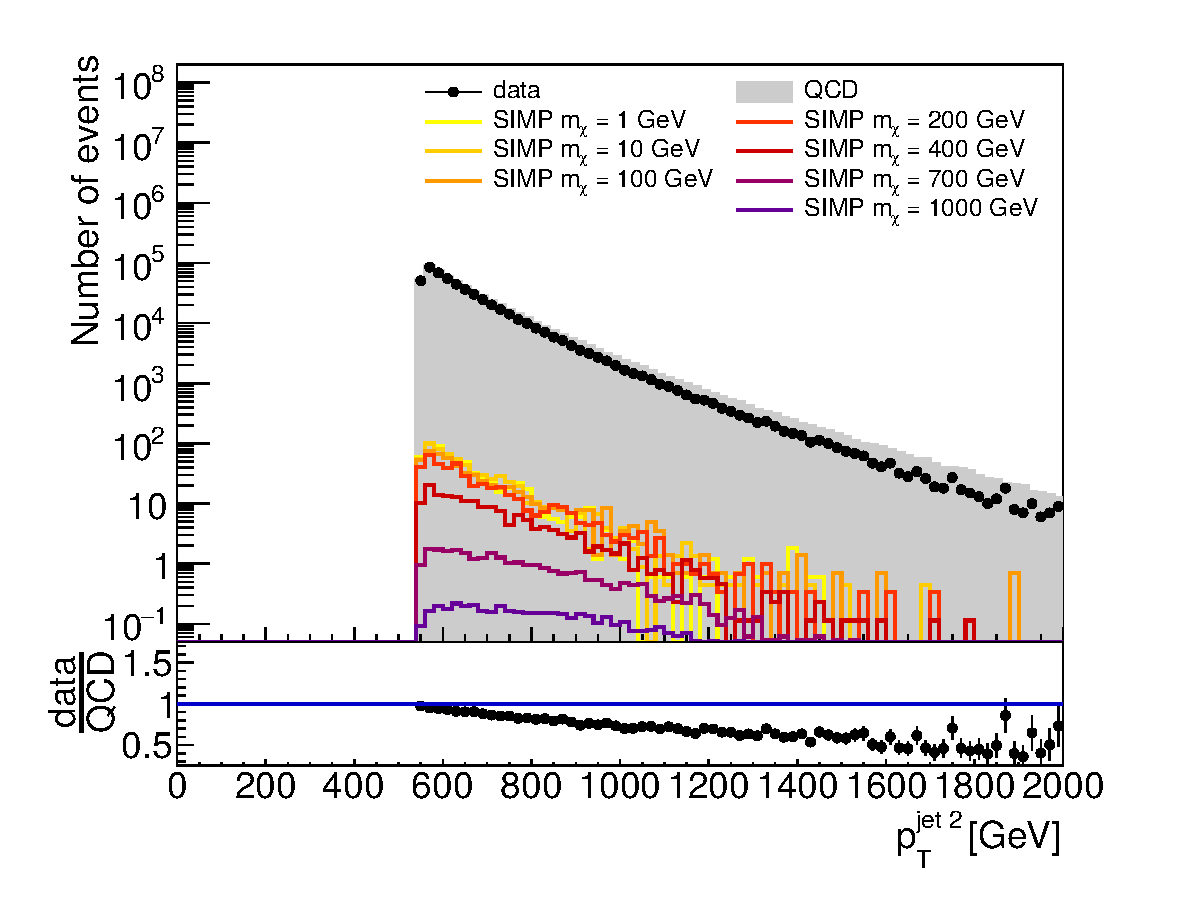
\includegraphics[width=0.5\textwidth]{figures/jet2_pt_newtrigger}
  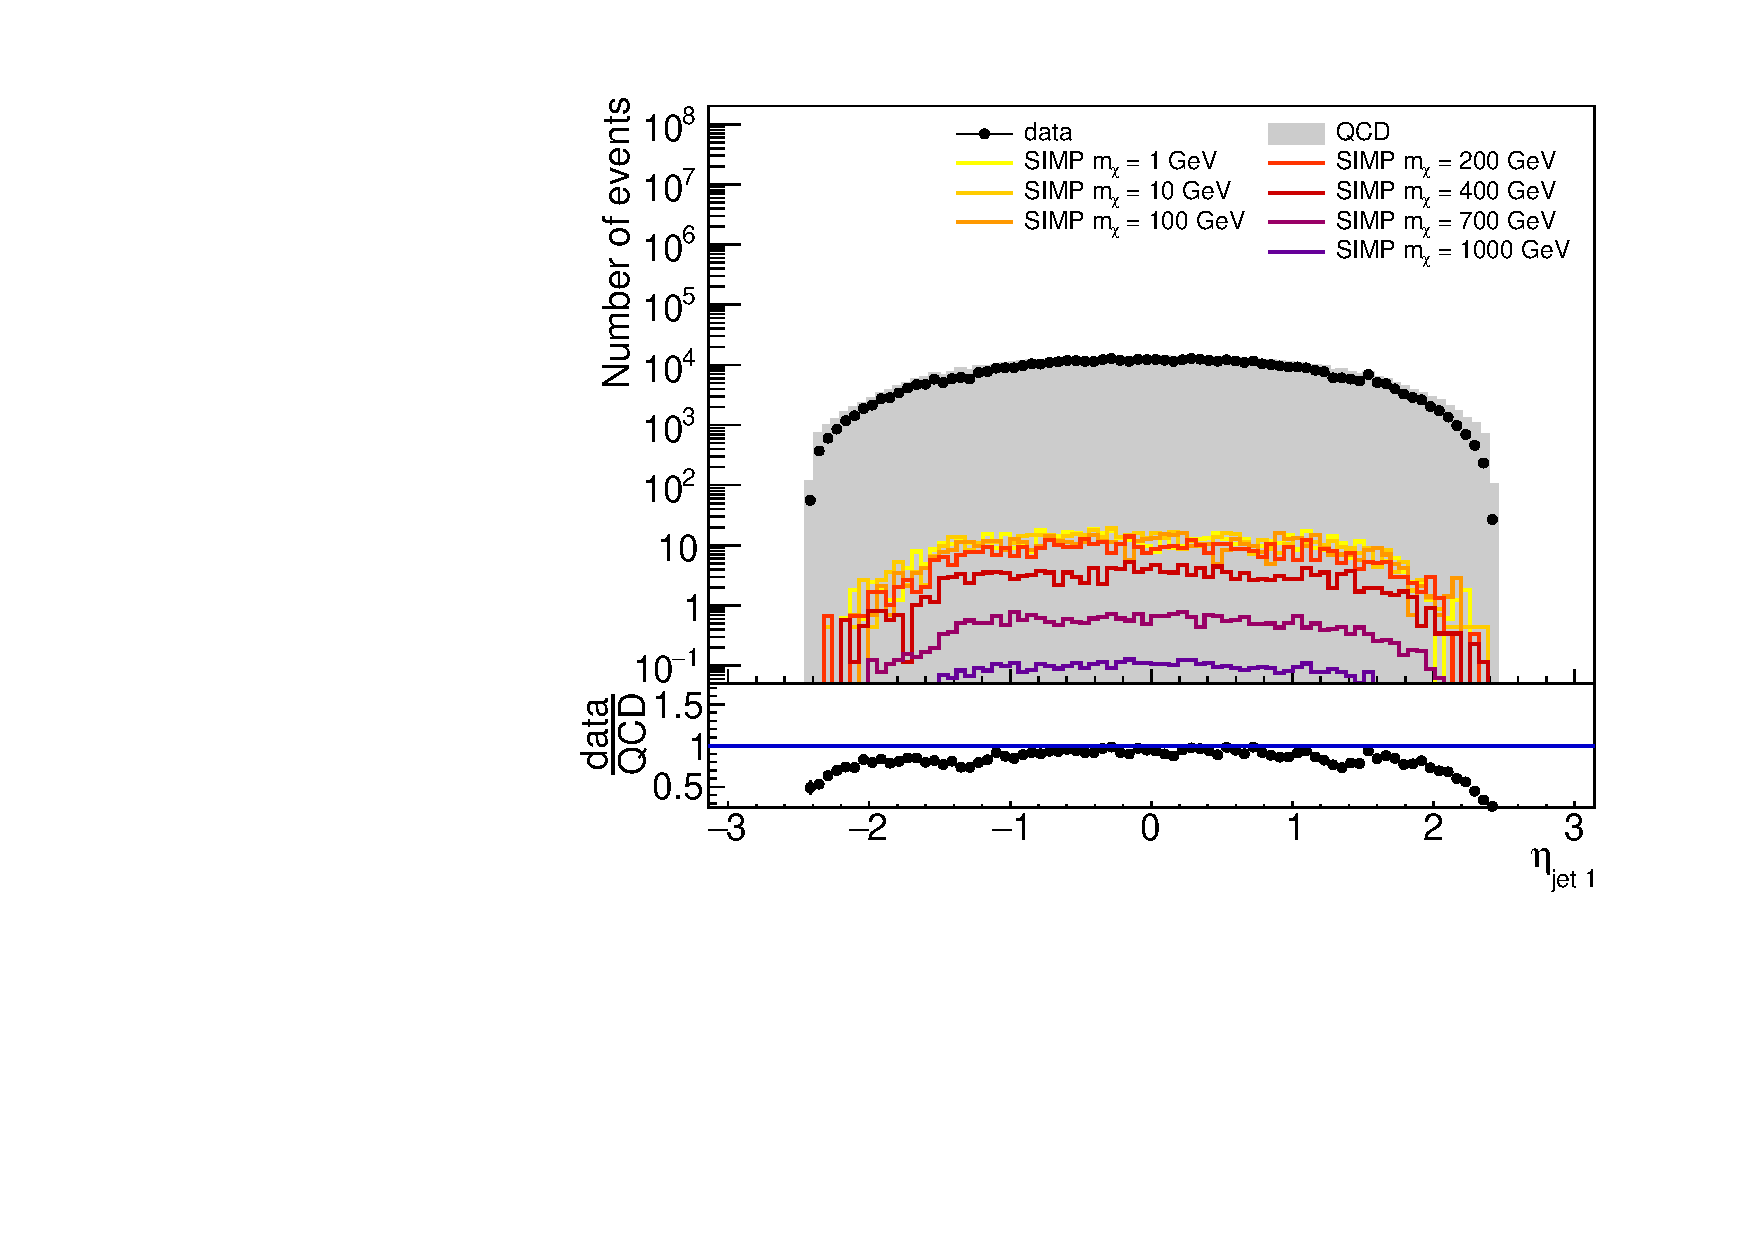
\includegraphics[width=0.5\textwidth]{figures/jet1_eta_newtrigger}\hfill%
  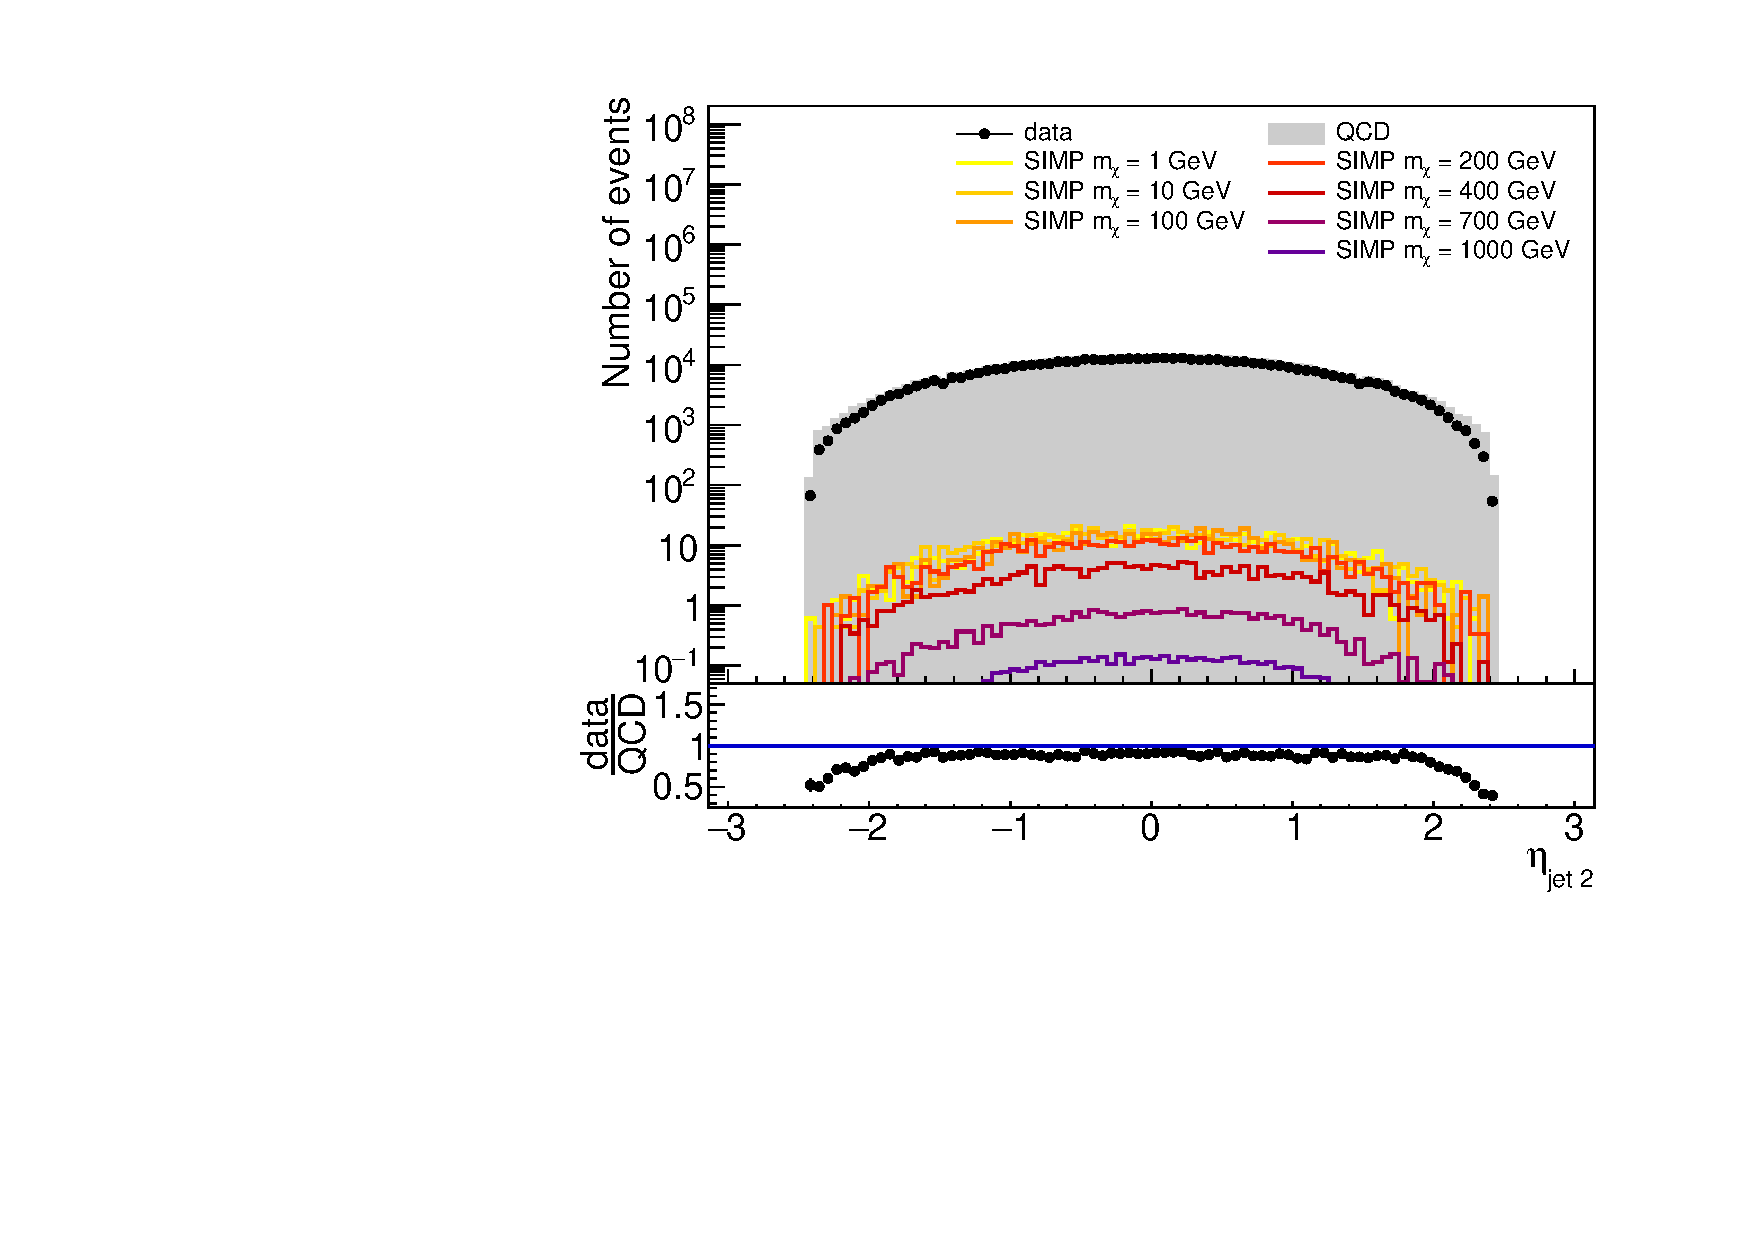
\includegraphics[width=0.5\textwidth]{figures/jet2_eta_newtrigger}
  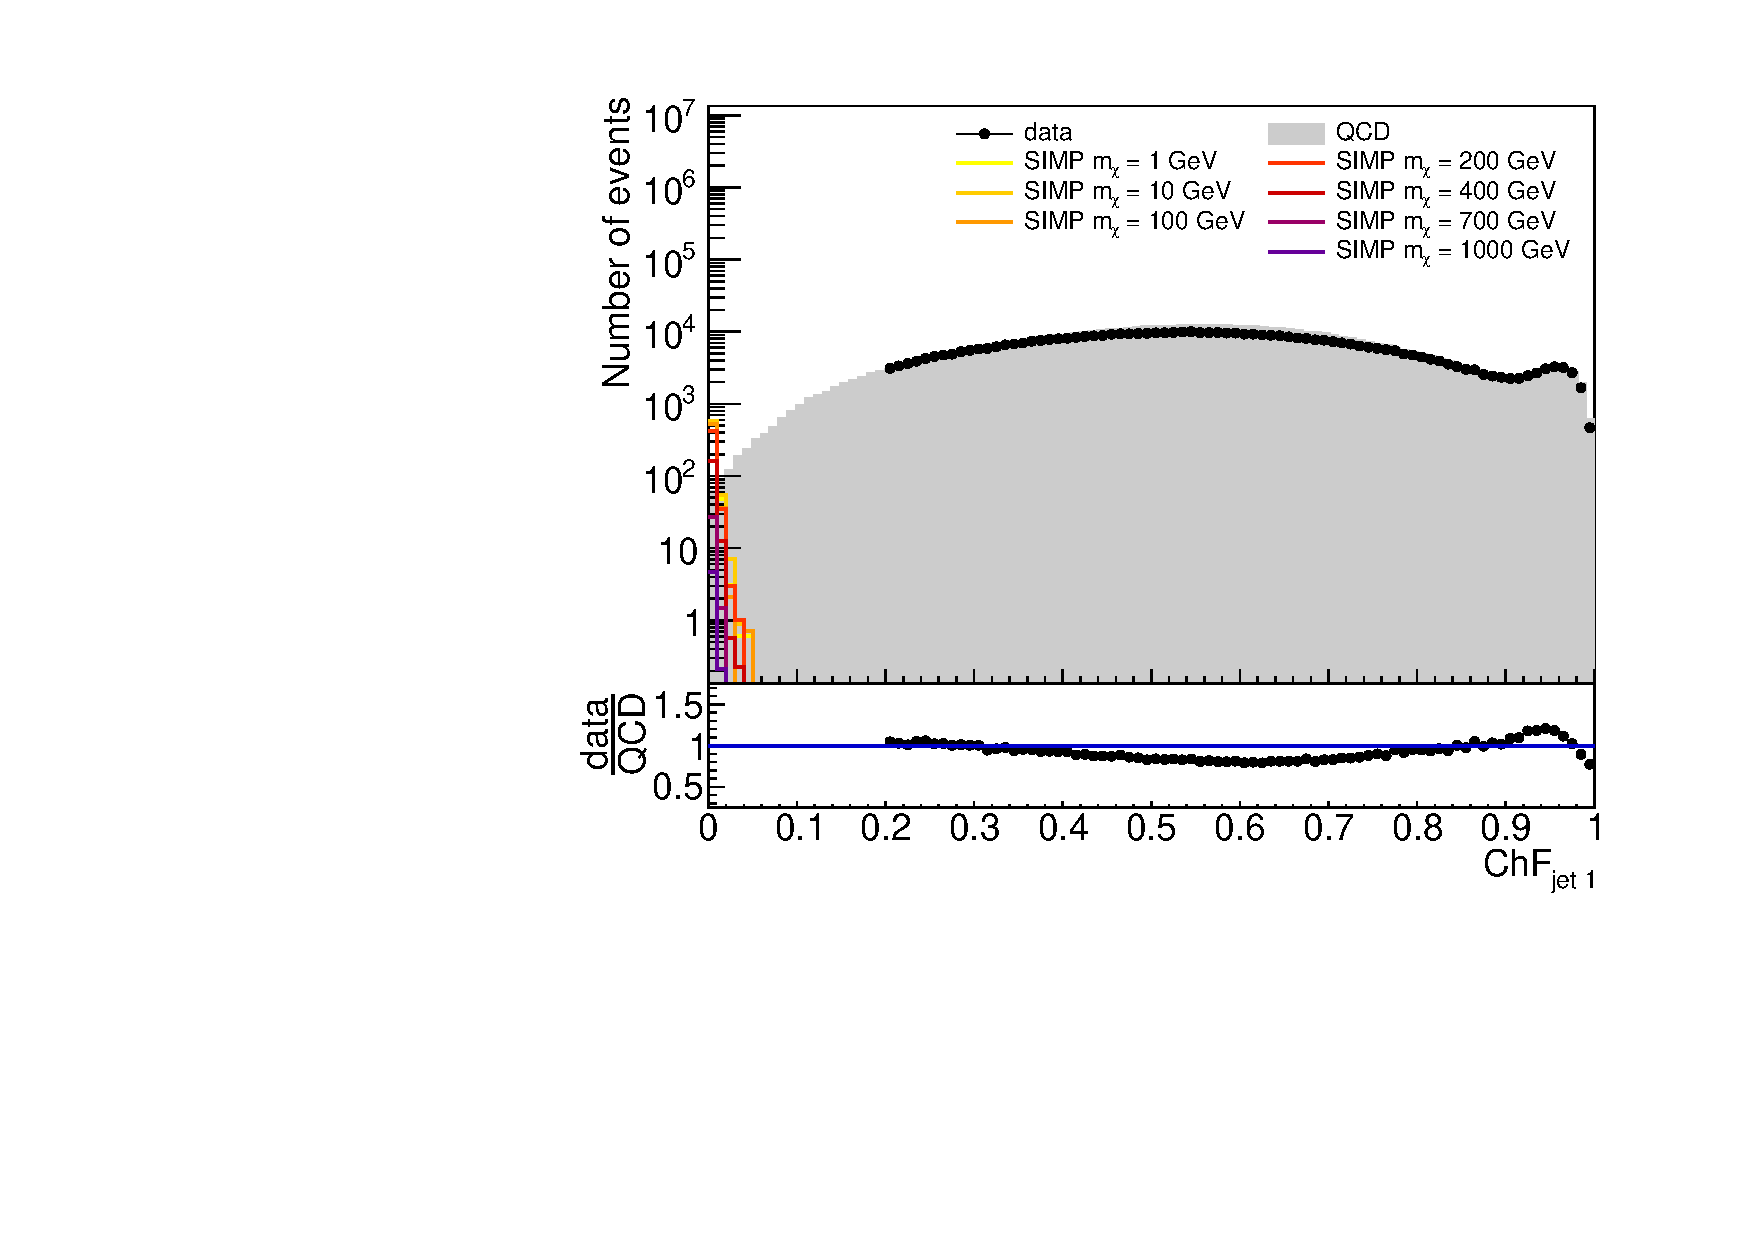
\includegraphics[width=0.5\textwidth]{figures/jet1_chf_newtrigger}\hfill%
  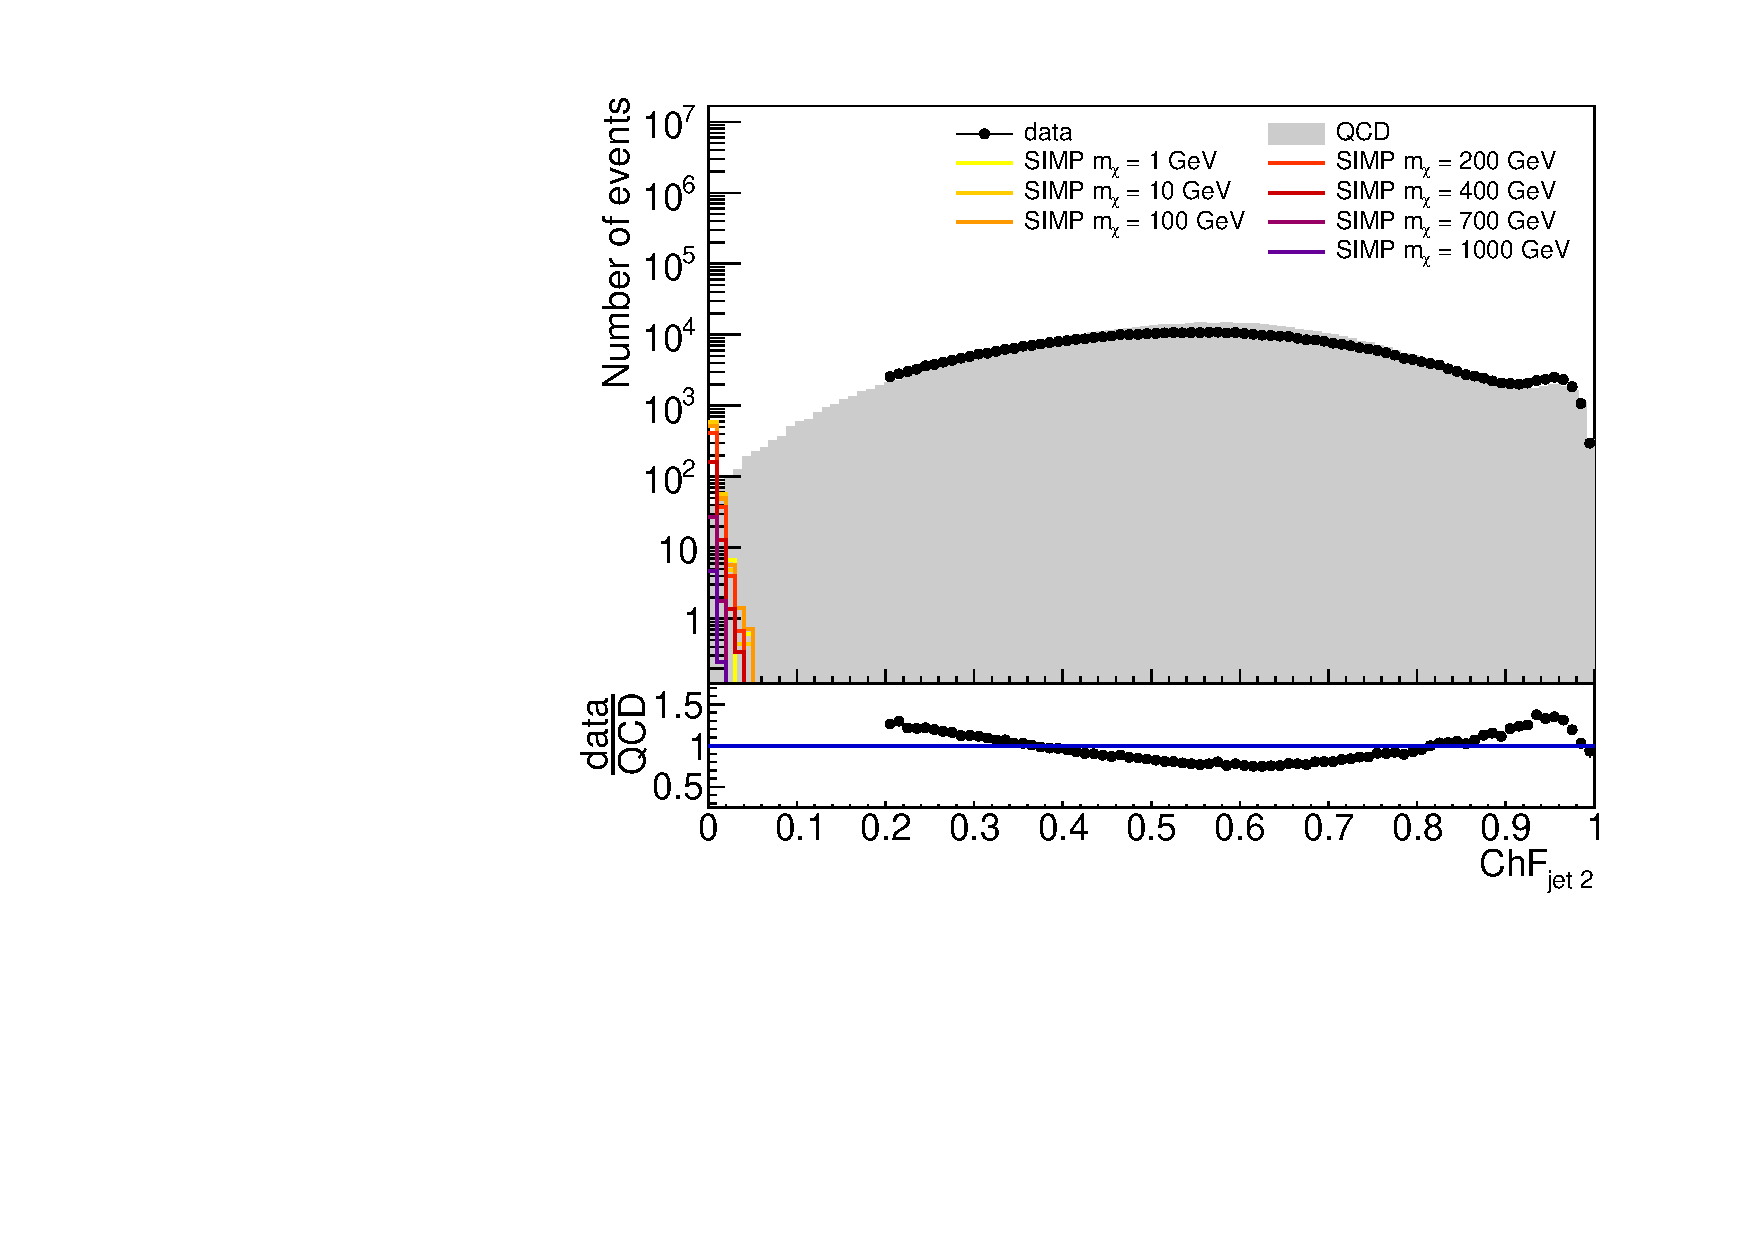
\includegraphics[width=0.5\textwidth]{figures/jet2_chf_newtrigger}
  \caption{$p_T$, $\eta$ and ChF of the leading (left) and subleading (right) jet. The selection cuts are applied, except for the cut on $\eta$ in the corresponding plot.}
  \label{fig:event_selection}
\end{figure}

\begin{figure}[h]
  \centering
  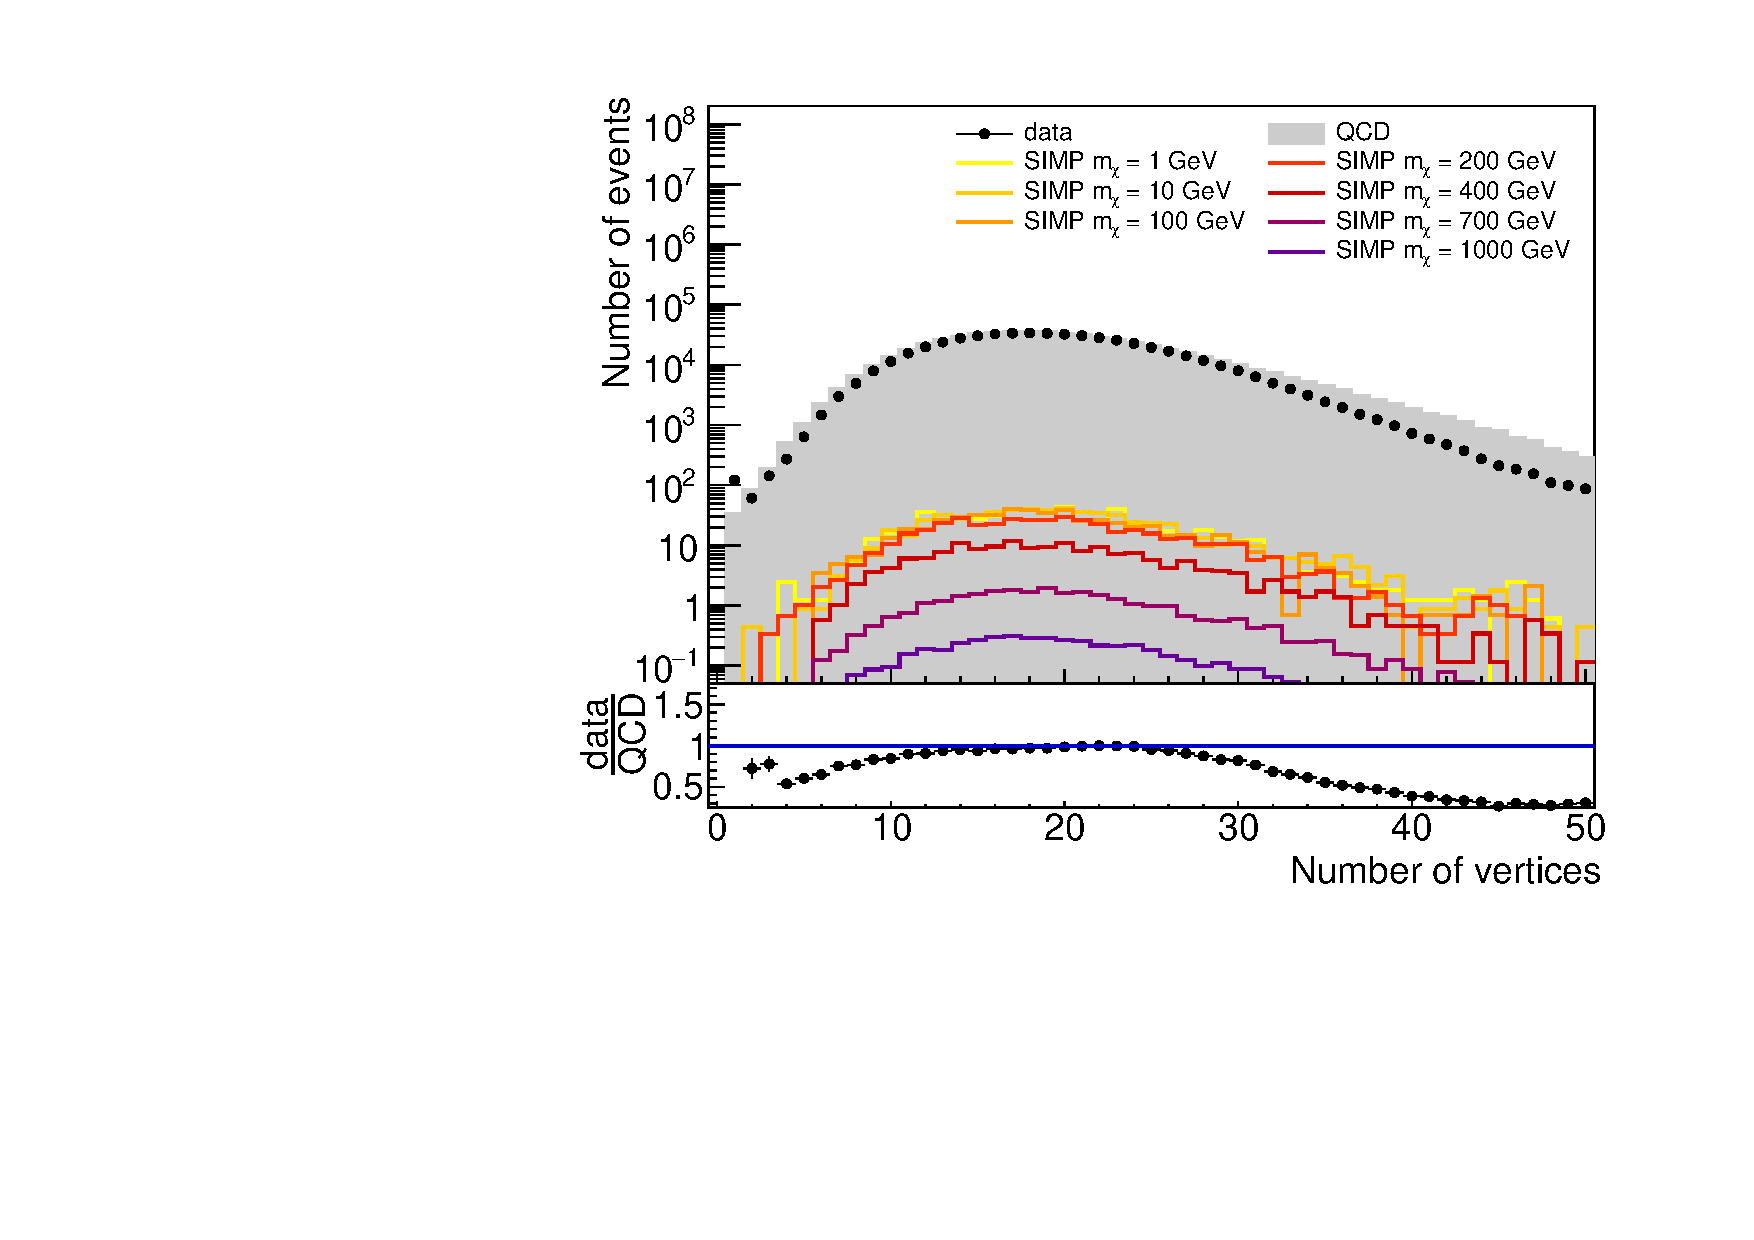
\includegraphics[width=0.5\textwidth]{figures/nvtx_newtrigger}\hfill%
  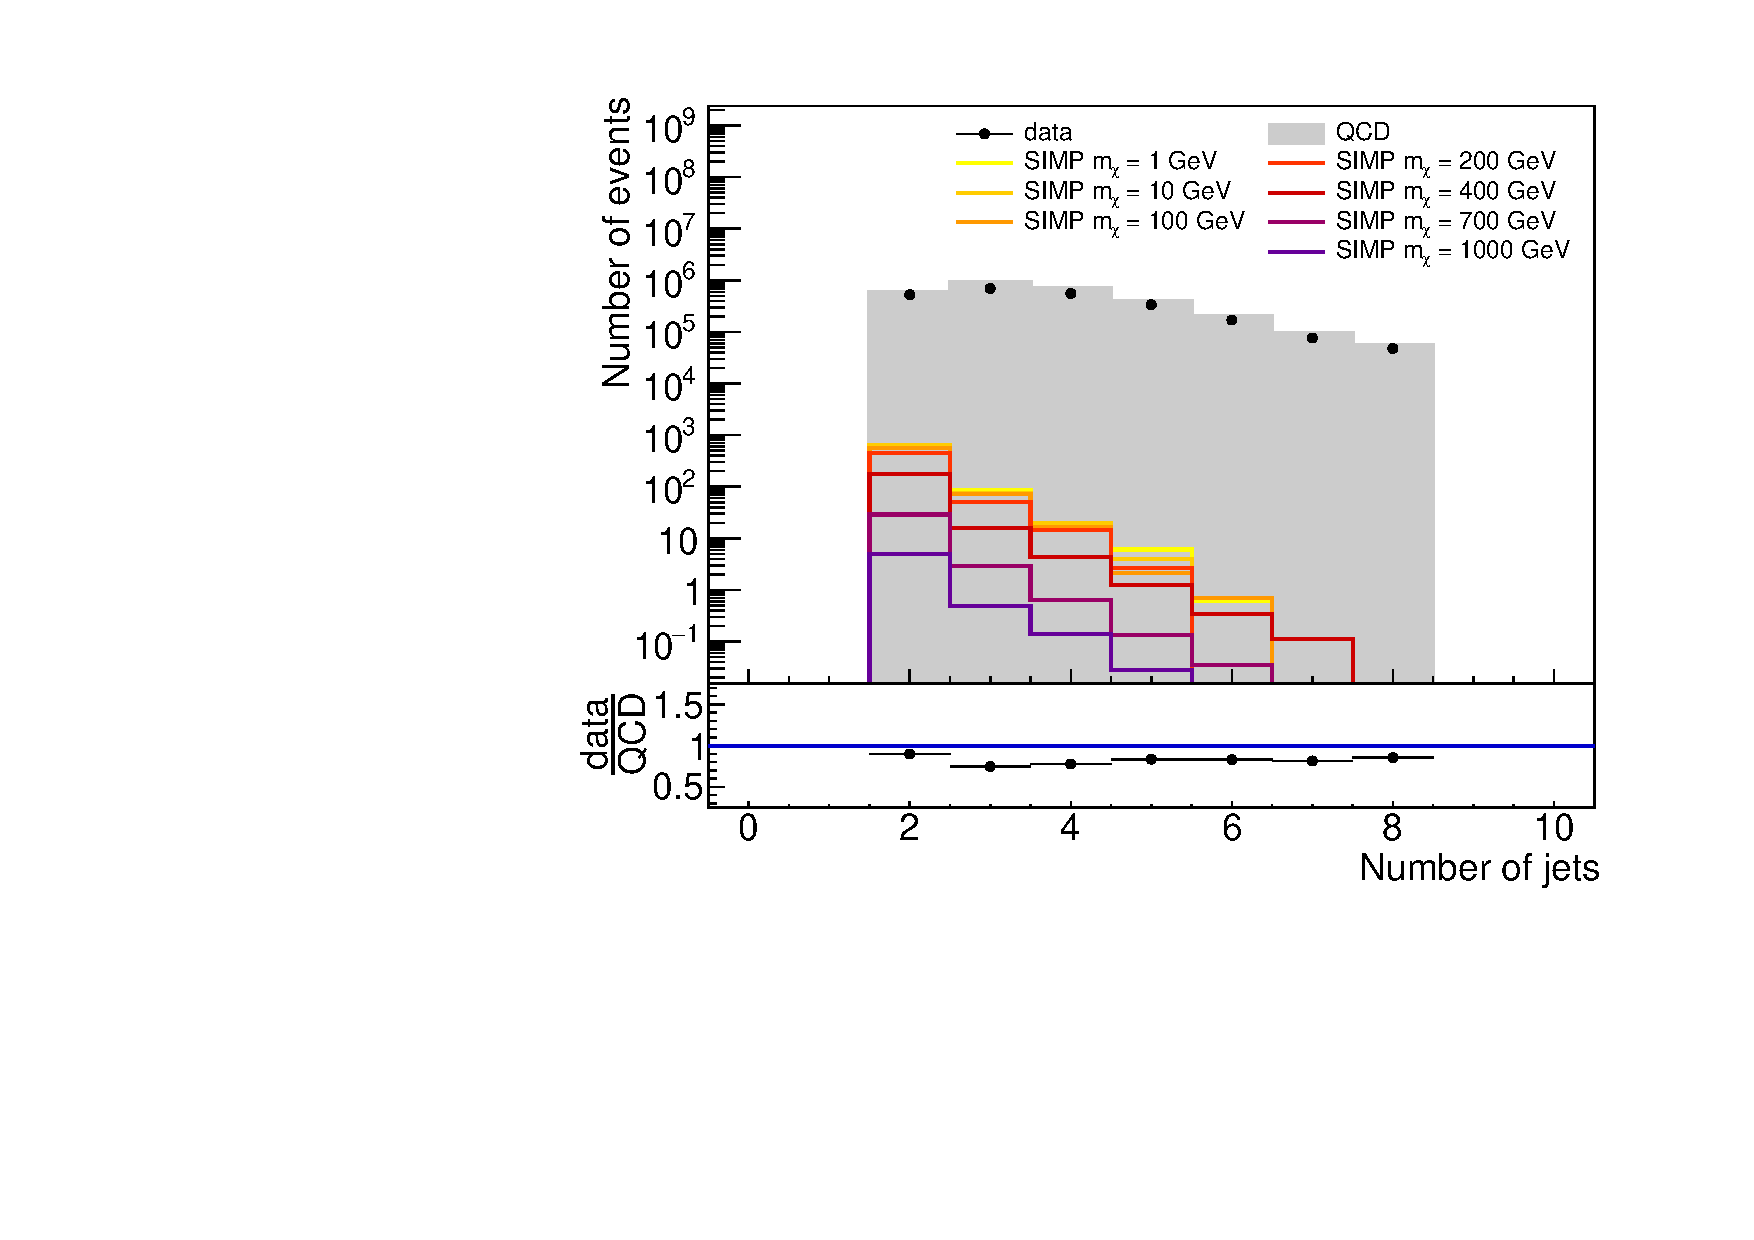
\includegraphics[width=0.5\textwidth]{figures/njets_newtrigger}
  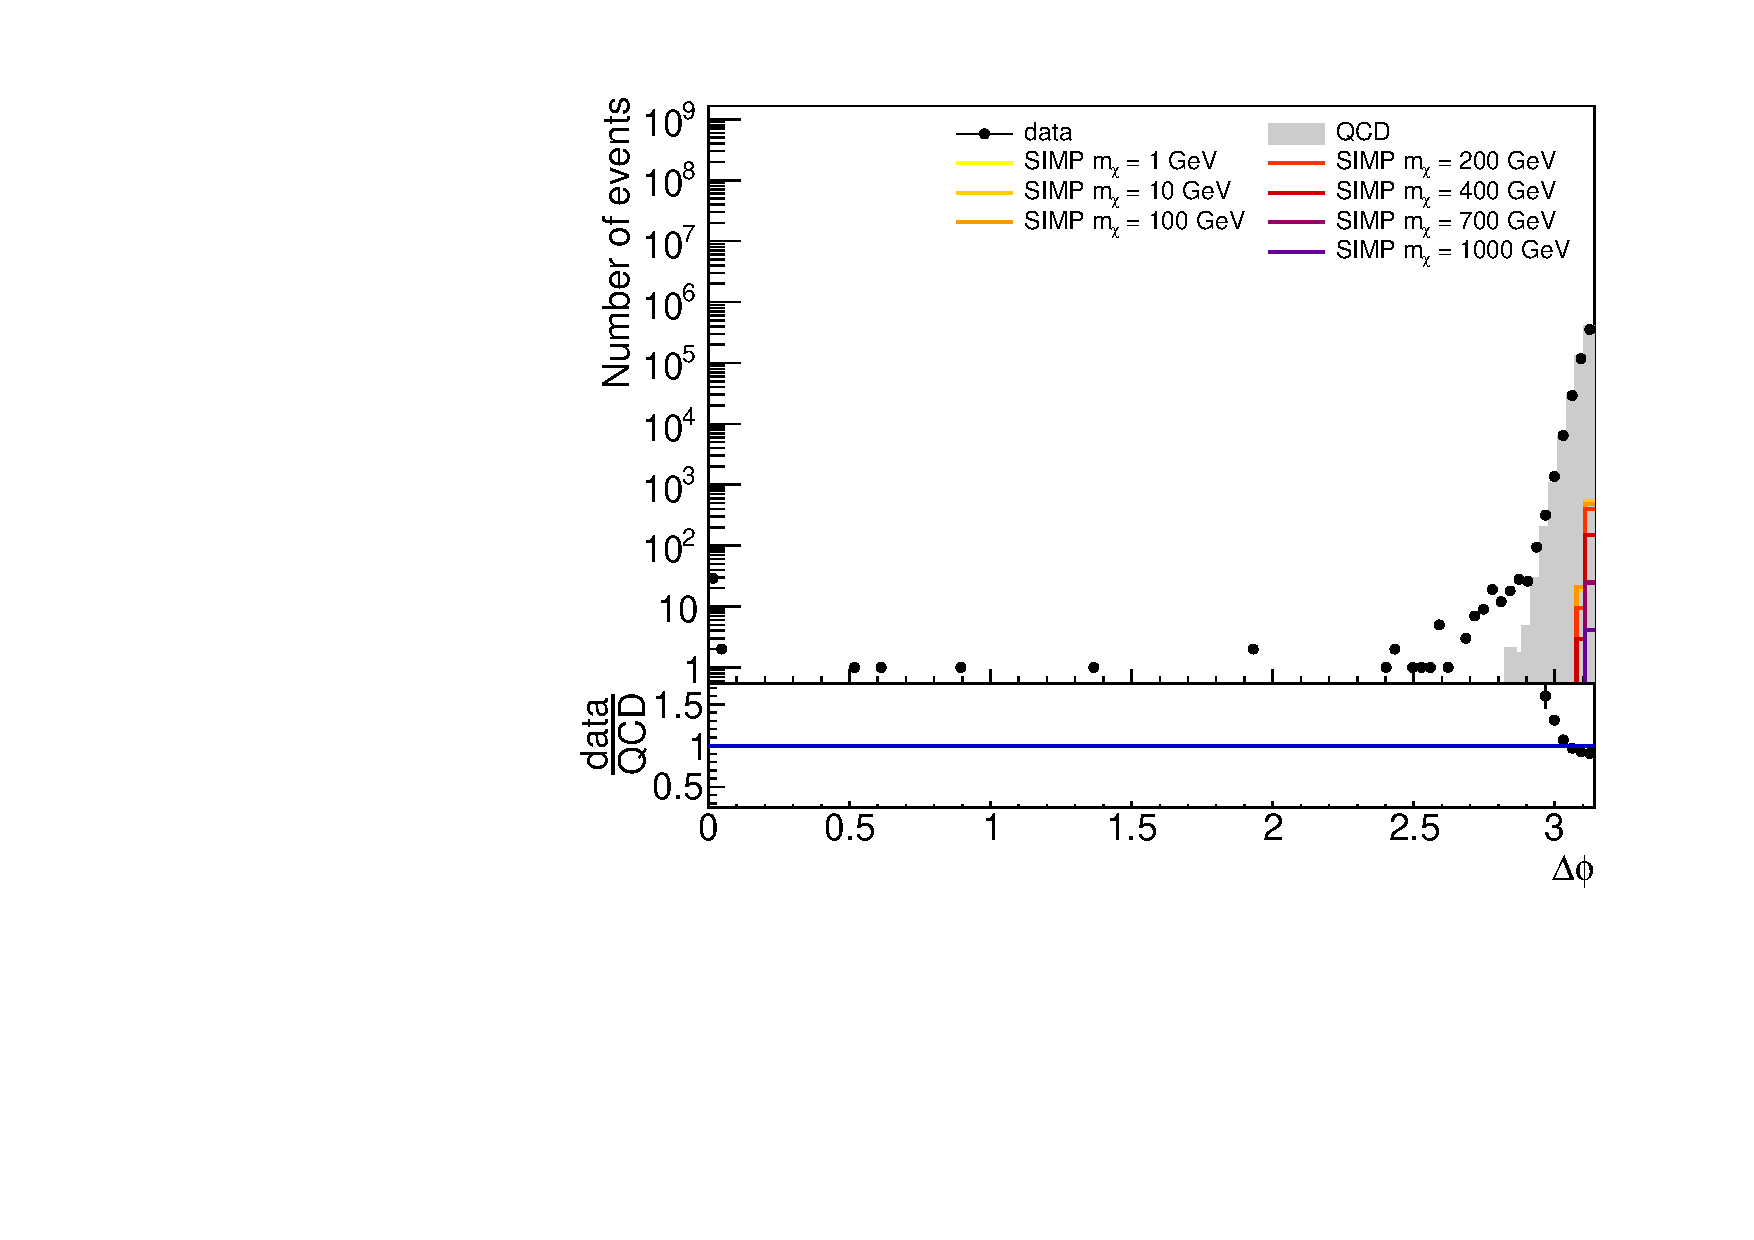
\includegraphics[width=0.5\textwidth]{figures/deltaphi}\hfill
  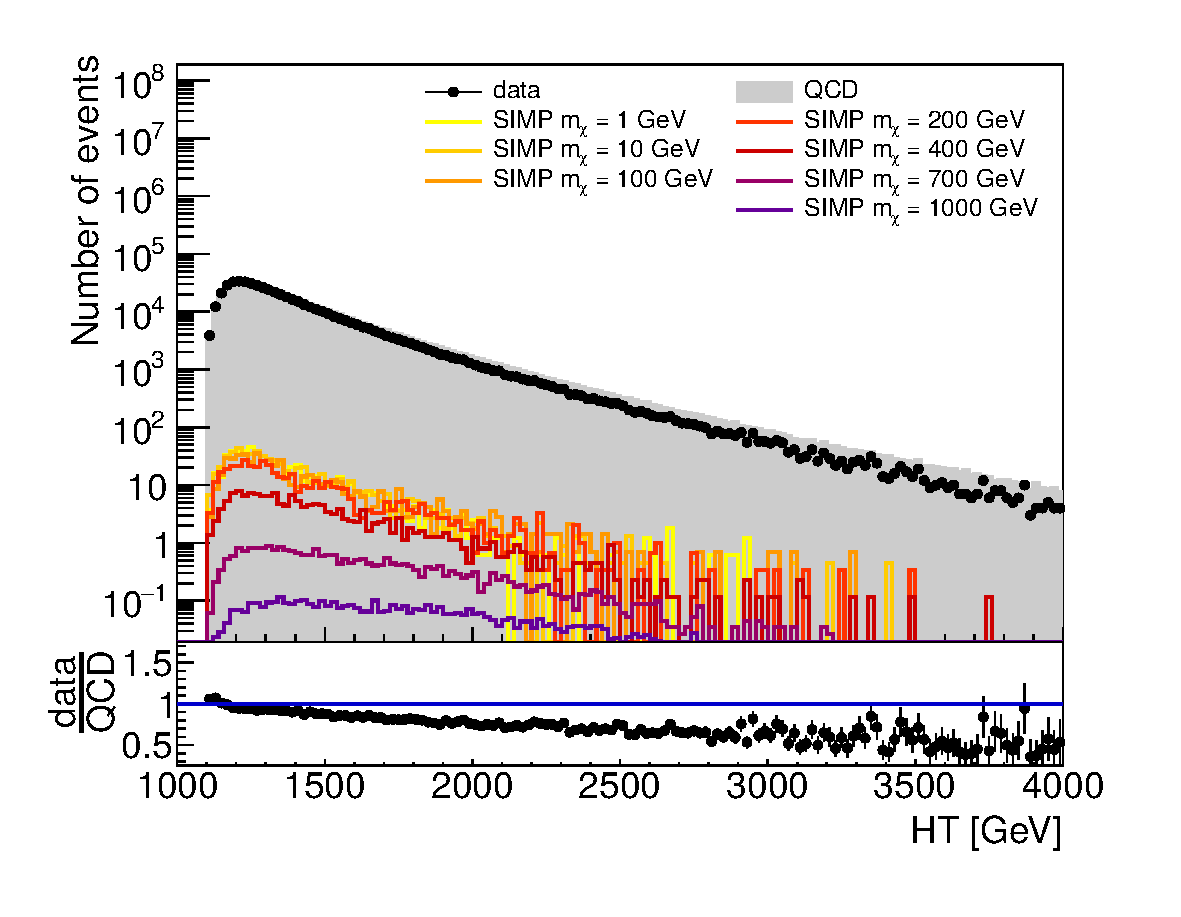
\includegraphics[width=0.5\textwidth]{figures/HT_newtrigger}
%  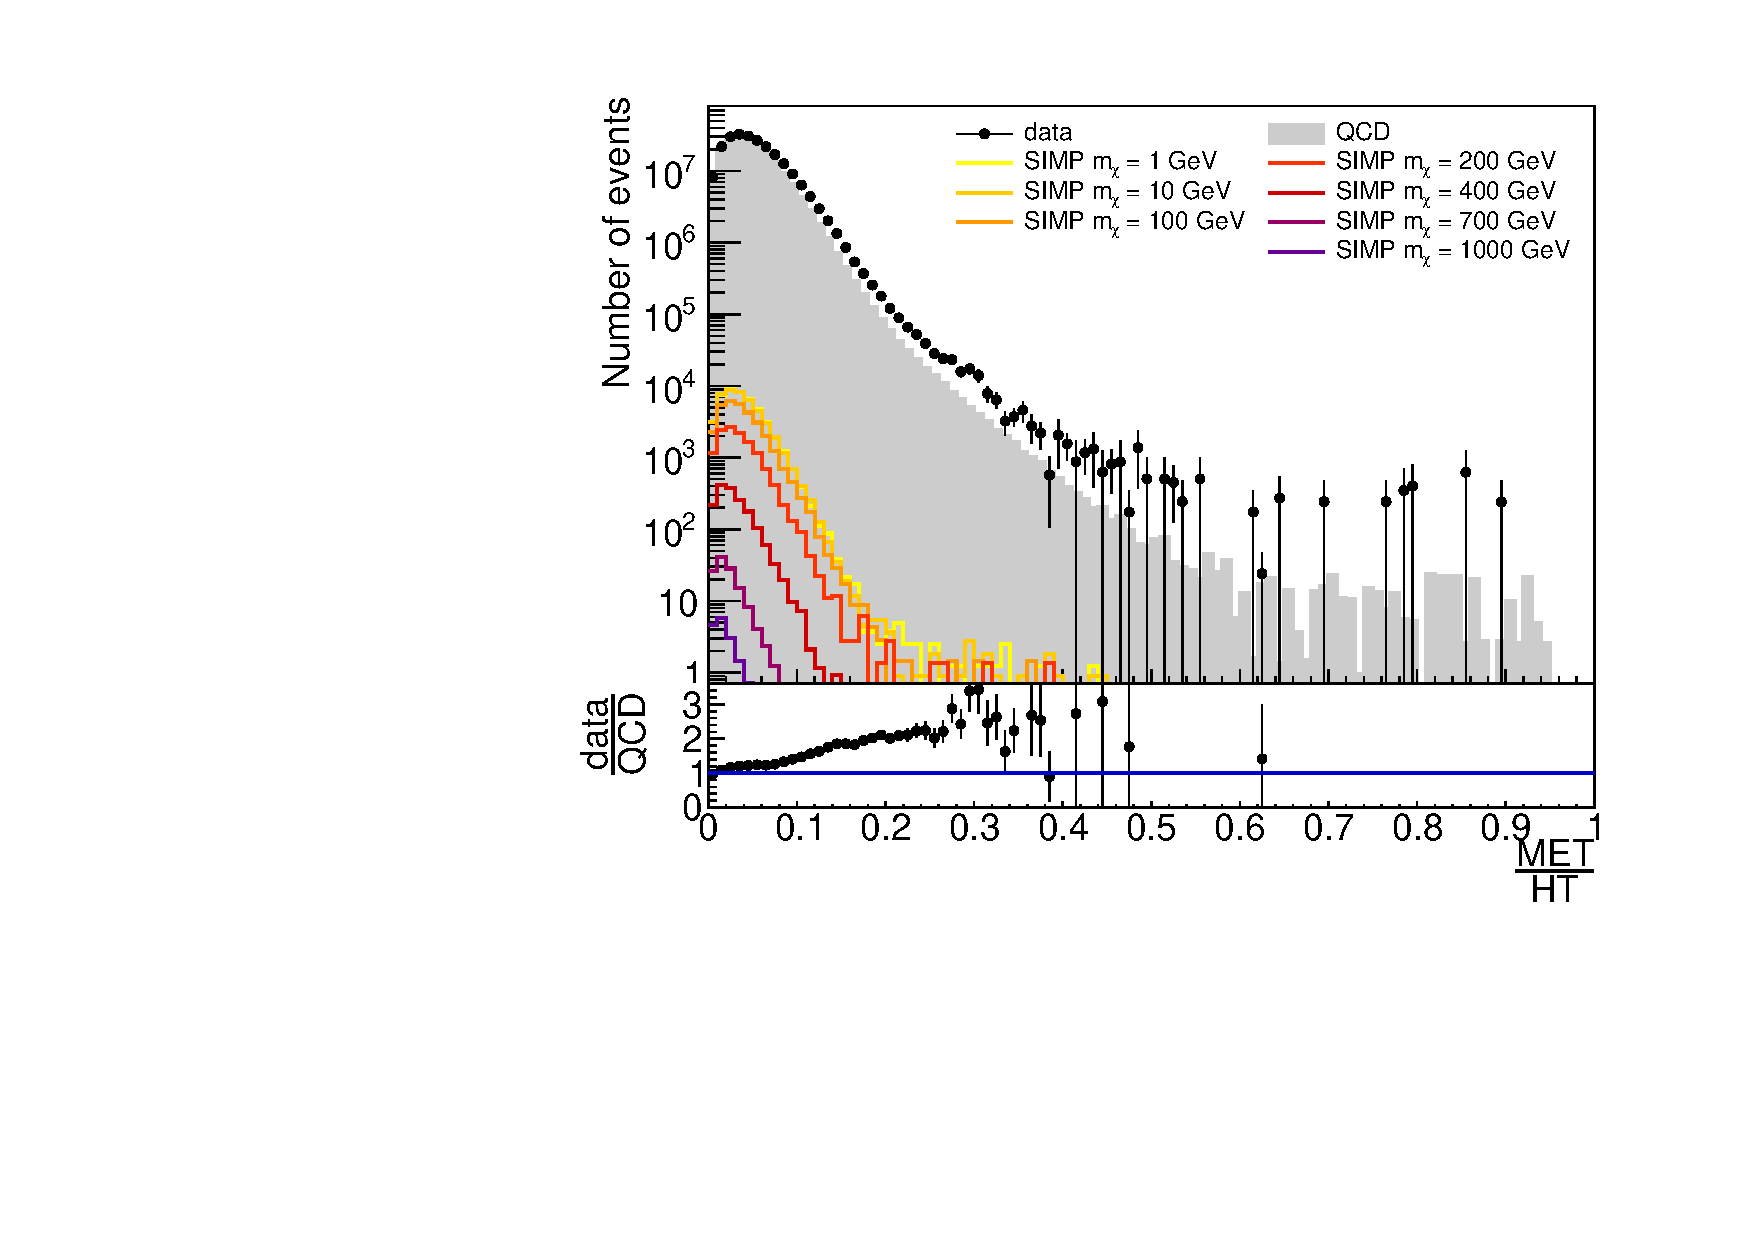
\includegraphics[width=0.5\textwidth]{figures/METOverHT} % wrong MET after P2PF.
  \caption{Number of vertices, number of jets, $\Delta\phi (\mathrm{jet}1, \mathrm{jet}2)$, and $H_{T}$ distributions, with selection cuts applied. The requirement on the number of vertices is not applied for the corresponding plot, the cut on the number of jets is not applied for the number of jets distribution, and the $\Delta\phi$ cut is similarly not applied for the corresponding distribution.}
  \label{fig:event_selection_2}
\end{figure}


\subsection{Control Region}

As will be detailed in Section~\ref{sec:SIMP_backgrounds}, the background is predicted from a data control region where one of the leading jets, or both, have a high ChF. The following selection is applied:

\begin{itemize}
 \item events pass the \texttt{HLT\_PFJet450} single jet trigger, as described in Section~\ref{sec:SIMP_trigger};
 \item leading and subleading jet have $p_T > \SI{550}{GeV}$ and $|\eta| < 2.0$;
%  \item $\Delta\phi > 2$ between leading and subleading jet;
 \item veto on additional jets;
 \item photon and conversion veto including a cut on the neutral EM energy fraction, as described above;
 \item at least two vertices are reconstructed;
 \item $\Delta\phi > 2$ between leading and subleading jet;
 \item events pass the MET filters;
 \item leading and/or subleading jet have ChF $> 0.25$.
\end{itemize}

No further selection on the second reconstruction with respect to the second primary vertex is applied here, since the presence of at least one jet with a large ChF avoids the problem of wrong selection of the primary vertex detailed in Section~\ref{sec:SIMP_reconstruction}.

\subsection{Signal region selection}

In the case of the signal region selection, we need to adapt the selection for the possible confusion of the primary vertex association. The selection looks as follows:

\begin{itemize}
 \item events pass the \texttt{HLT\_PFJet450} single jet trigger, as described in Section~\ref{sec:SIMP_trigger};
 \item leading and subleading jet have $p_T > 550$ GeV and $|\eta| < 2.0$;
%  \item $\Delta\phi > 2$ between leading and subleading jet;
 \item veto on additional jets;
 \item photon and conversion veto including a cut on the neutral EM energy fraction, as described above;
 \item at least two vertices are reconstructed;
 \item $\Delta\phi > 2$ between leading and subleading jet;
 \item events pass the MET filters;
 \item ChF $< x$, where $x$ is the signal cut being considered. In this case, we apply the cut on the leading as well as subleading jet, for both reconstructions starting from the first and second primary vertex.
\end{itemize}

The values for $x$ considered in this analysis defining the signal regions are 0.03, 0.04, 0.05, 0.1, 0.15, and 0.2. 

\section{Background estimation}
\hspace{1cm}
{\color{red} TODO}

\subsection{Photon + jets}

The photon + jets background was verified to be negligible and well within any other systematic uncertainty on the background prediction. The photon veto is found to work well, especially the cut on the jet neutral electromagnetic fraction, and no events from the used MC sample remain after applying a cut of ChF $<$ 0.1. Additionally, the events remaining just above that cut are partly contained in the overlapping QCD multijets sample.

\subsection{QCD multijets}

The QCD multijet background is estimated from data, since the MC does not describe the data well, especially at low ChF, as can be seen from Figure~\ref{fig:dataMC} which compares the ChF distribution in the control region to the QCD MC. In this plot the subleading jet is required to have a large ChF, in order to stay blind in data.

\begin{figure}[h]
  \centering
  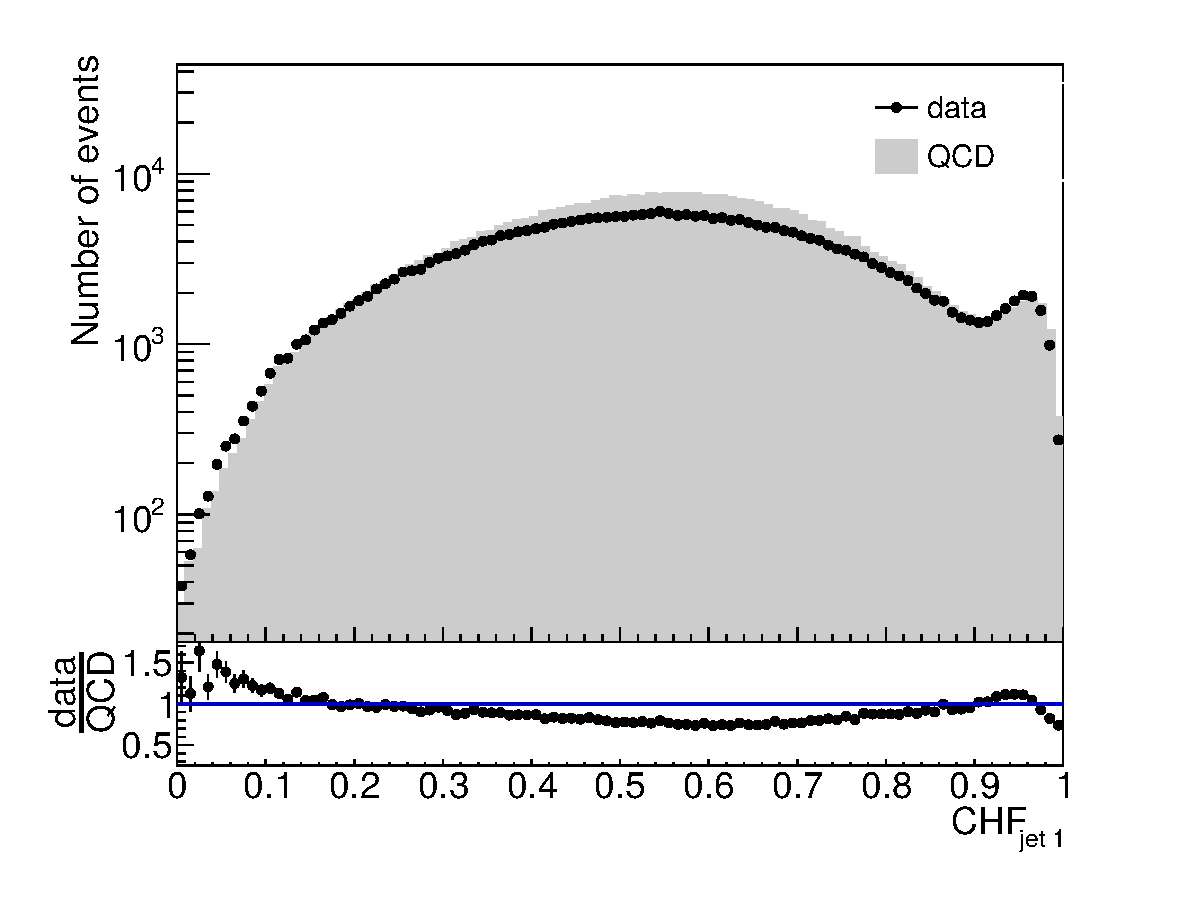
\includegraphics[width=0.7\textwidth]{figures/bkgd_estimation_dataMC.pdf}\hfill%
  \caption{Data-MC comparison of the charged energy fraction of the leading jet, tagging events with subleading jet ChF $>$ 0.5.}
  \label{fig:dataMC}
\end{figure}

As a first step, we measure the efficiency of the ChF cut in the control region, by requiring one jet to have large ChF (ChF $>$ 0.25) and applying the ChF cut on the other jet. The measurement was done in bins of jet $p_T$ and $\eta$. The number of QCD events in the signal region is then predicted by using any QCD dijet event passing the selection cuts listed in Table~\ref{tab:cutflow} and applying the appropriate $p_T$ and $\eta$ dependent ChF cut efficiencies on the 2 leading jets. Figure~\ref{fig:efficiencies} shows the measured 1D efficiency as a function of the ChF cut for various bins in $p_T^{jet}$ and $\eta_{jet}$, as measured in MC. There is a strong dependence on the jet $p_T$, and a less pronounced dependence on the jet $\eta$ at low ChF. The efficiencies are the highest for the $1.0 < |\eta| < 1.25$ bin, which can be attributed to this being the barrel-endcap transition region where most of the tracker material budget is located. The dependence on the jet $p_T$ arises from the reconstruction. As can be seen from the left plot in Figure~\ref{fig:pt_dependence}, at generator level the ChF is independent of the jet $p_T$, as one would expect. After reconstruction, as demonstrated in the right plot of Figure~\ref{fig:pt_dependence}, a $p_T$ dependence arises due to the known degradation of tracking efficiency in dense jet environments, which becomes more of an issue for very high $p_T$ and thus collimated jets.

\begin{figure}[h]
  \centering
  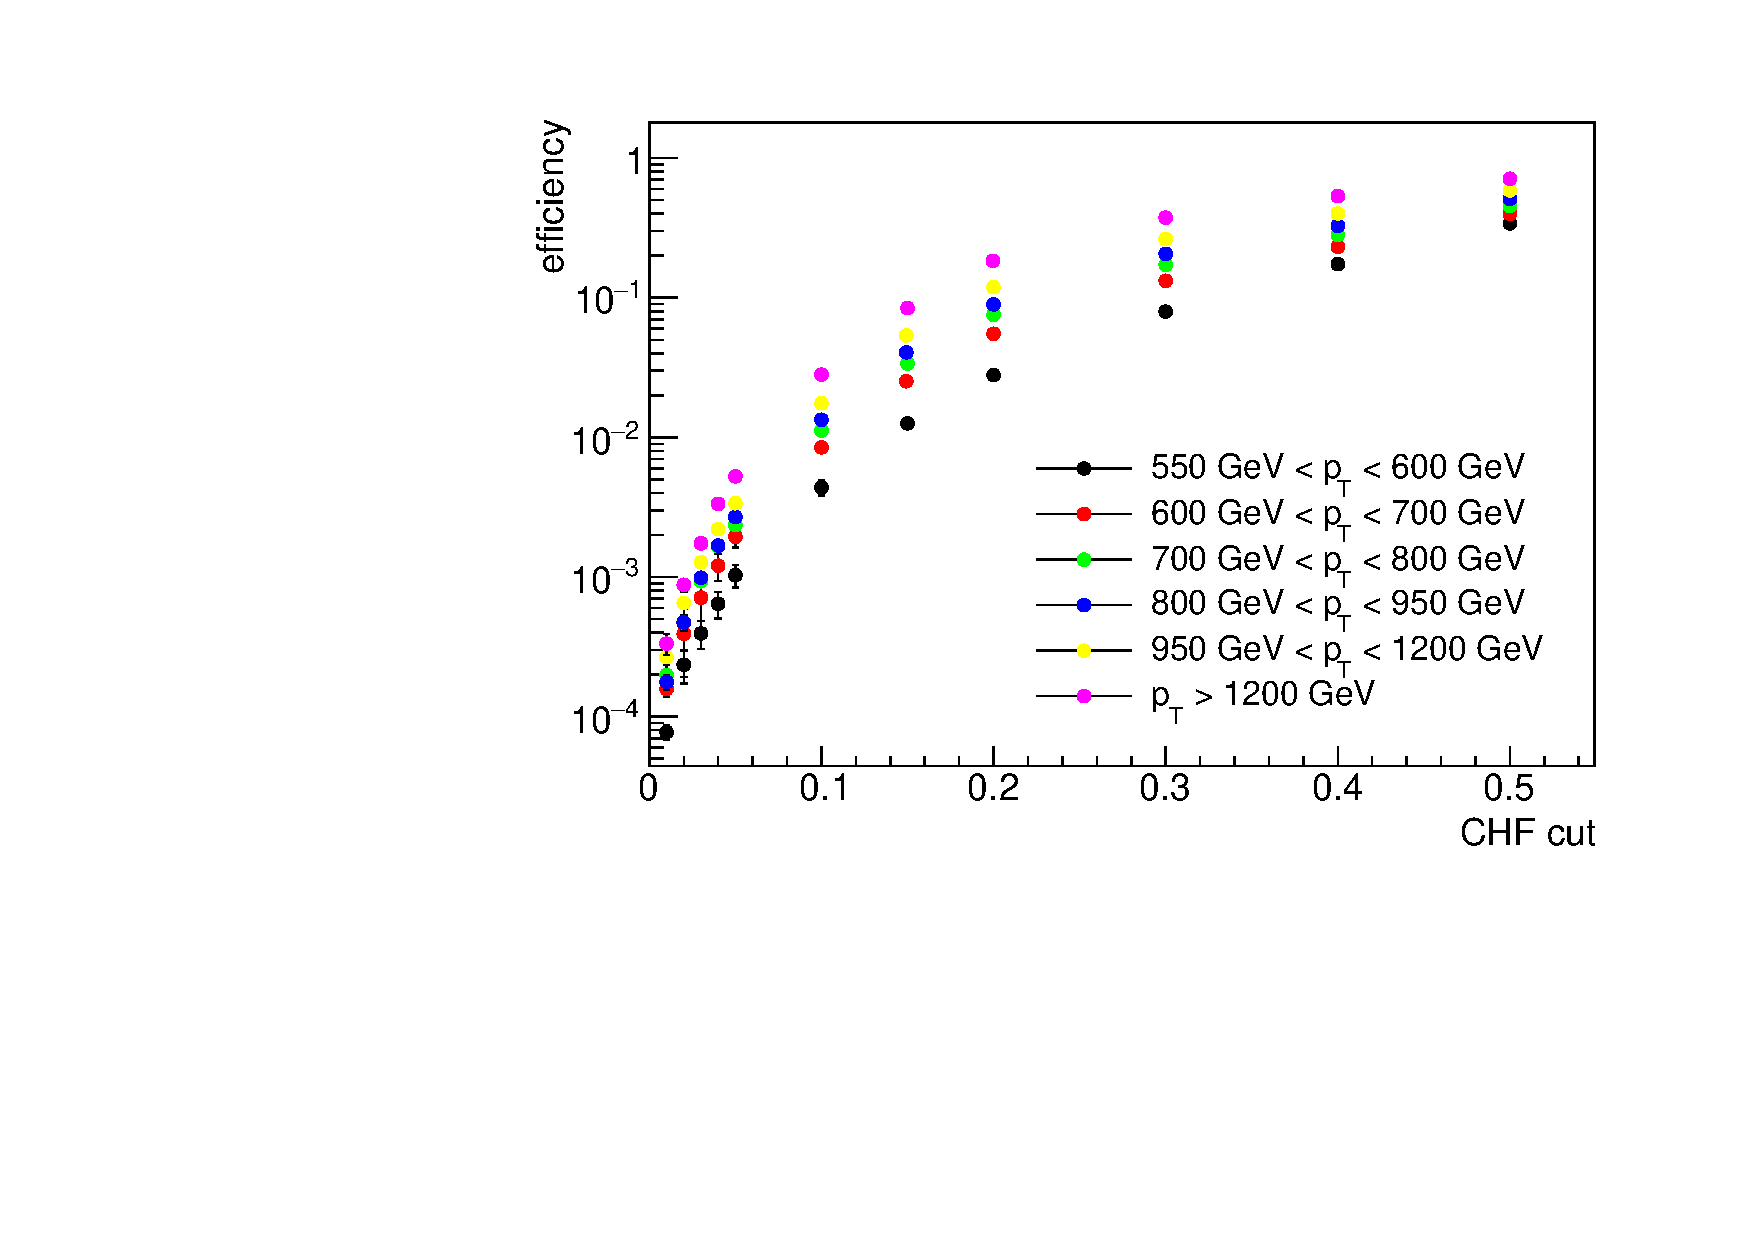
\includegraphics[width=0.5\textwidth]{figures/eff1D_pt_newtrigger.pdf}\hfill%
  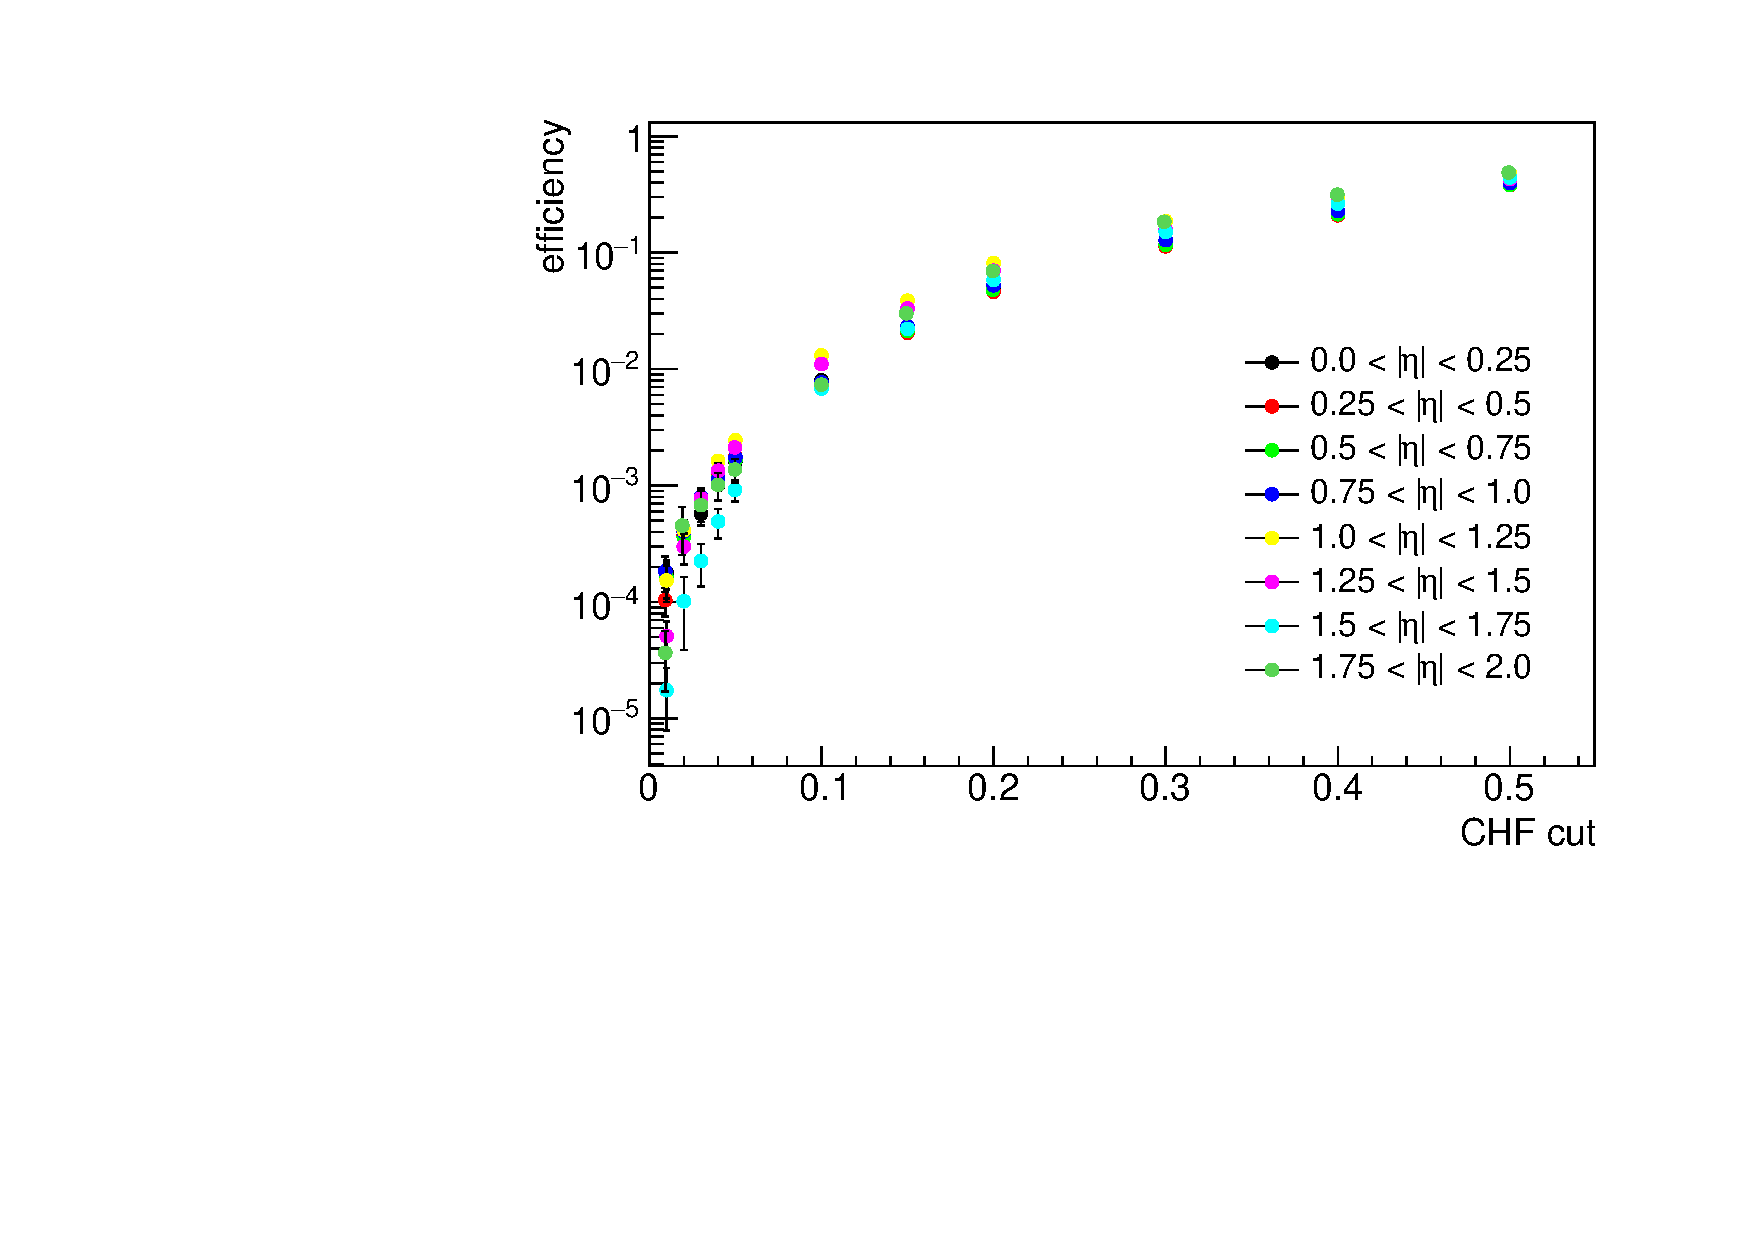
\includegraphics[width=0.5\textwidth]{figures/eff1D_eta_newtrigger.pdf}
  \caption{The efficiency of several ChF cuts in QCD MC, binned in $p_T$ (left) and $\eta$ (right).}
  \label{fig:efficiencies}
\end{figure}

\begin{figure}[h]
  \centering
  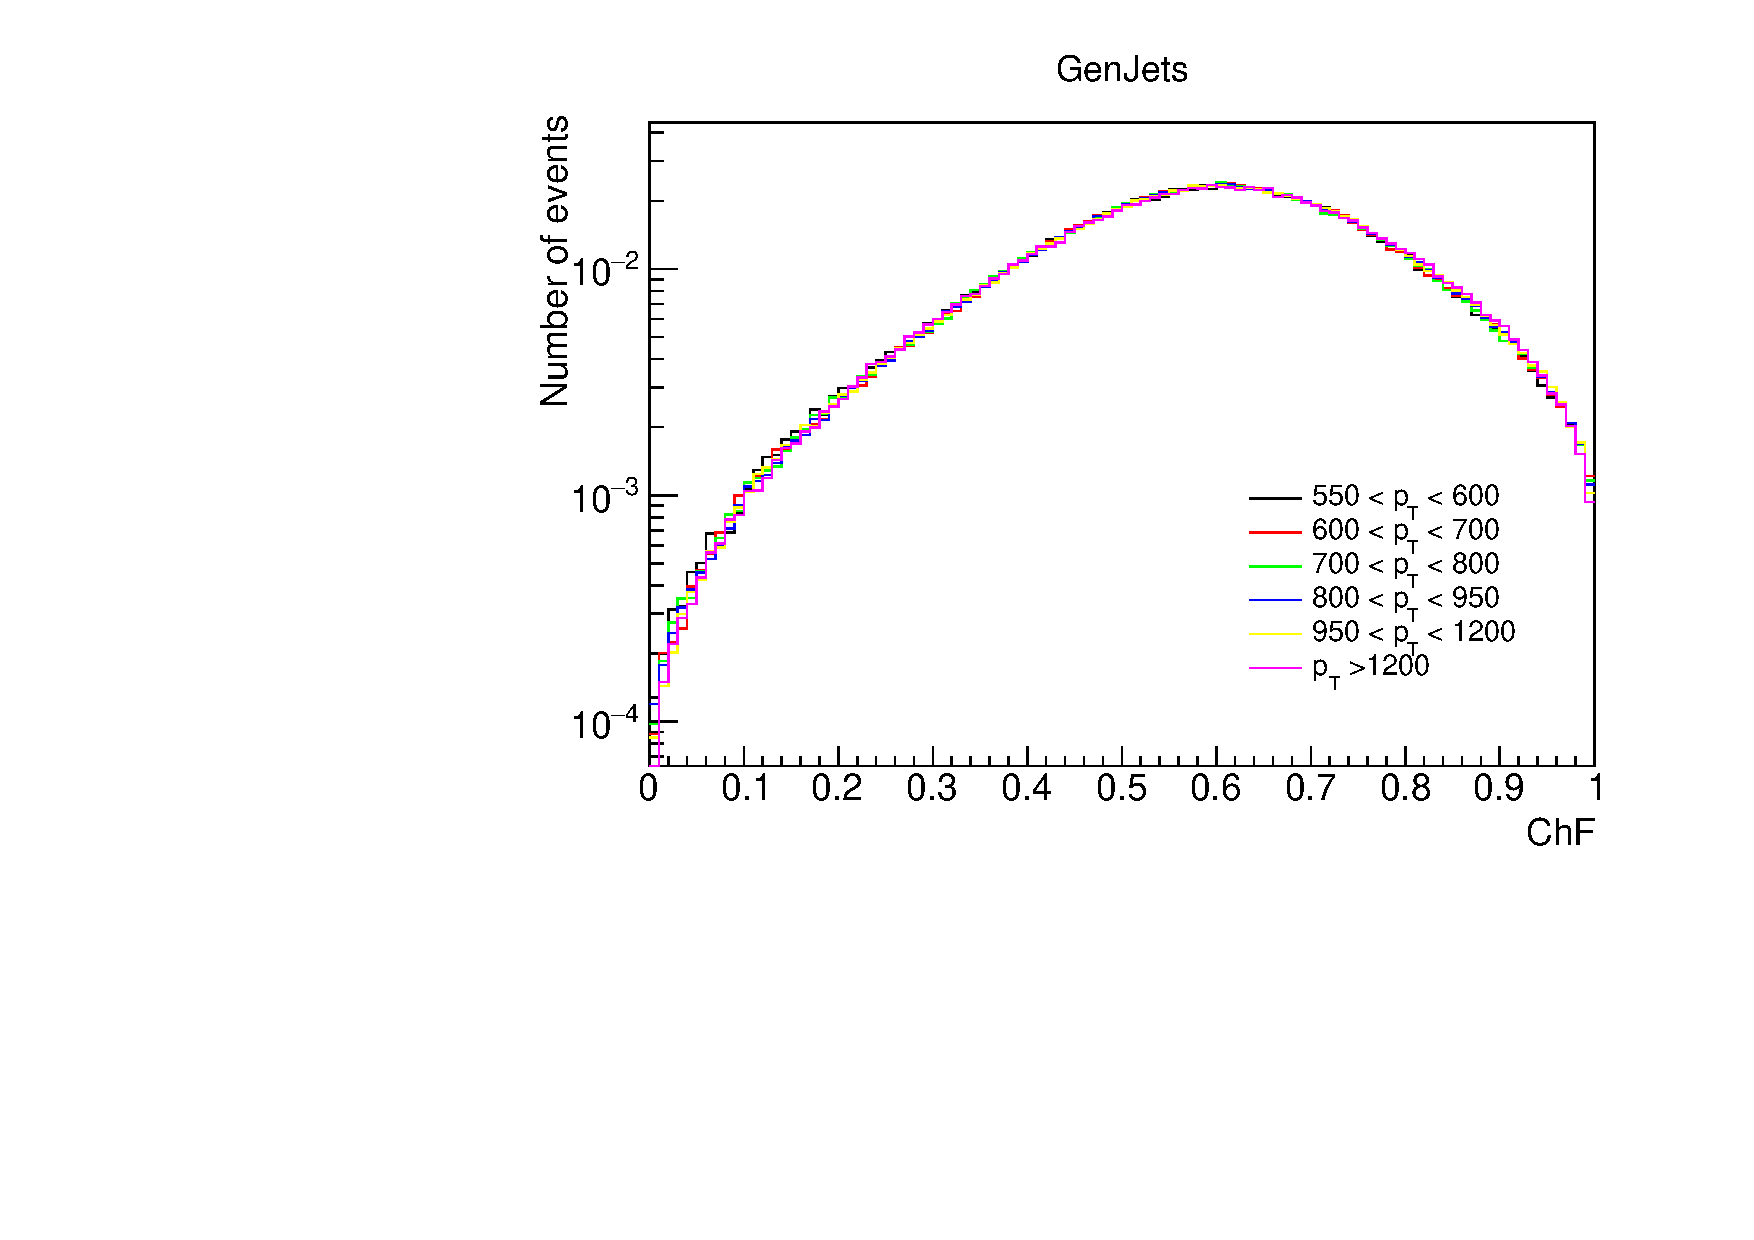
\includegraphics[width=0.5\textwidth]{figures/ChFPerPtbin_GenJets.pdf}\hfill%
  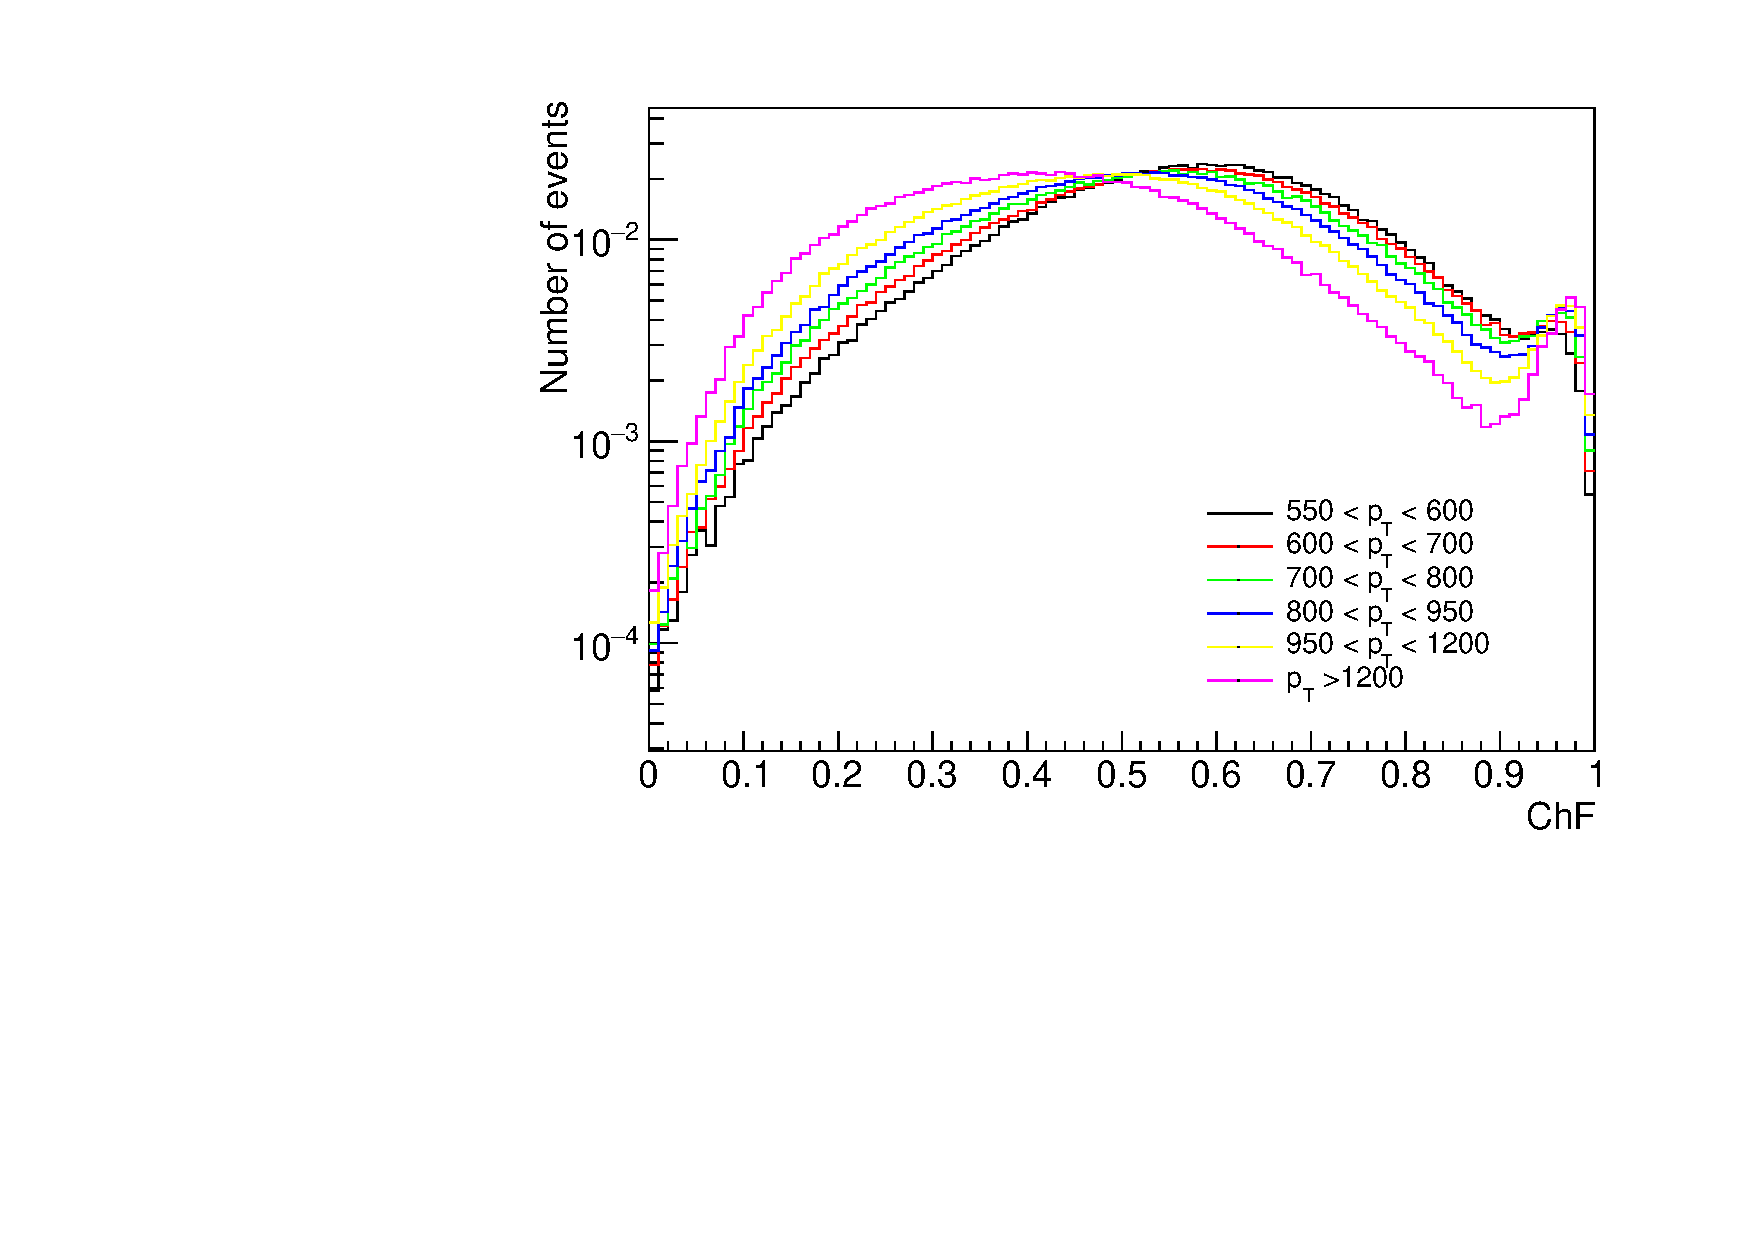
\includegraphics[width=0.5\textwidth]{figures/ChFperPtbin.pdf}
  \caption{The ChF per bins of jet $p_T$, for generator level (left) and reconstructed (right) jets.}
  \label{fig:pt_dependence}
\end{figure}

A closure test is performed to validate this background prediction method, by comparing the MC truth and the 1- and 2-leg predictions in MC. The MC truth shows the yield after applying the ChF cuts on both jets. For the 1-leg prediction the ChF cut is applied on one jet and the event is then scaled by the measured $$p_T$$- and $\eta$-dependent efficiency for the other jet. For the 2-leg prediction, the efficiencies are applied for both jets, and no ChF cut is applied directly.

As a first check the closure test was also performed at the generator level, using GenJets. This comparison is done in exclusive bins in (ChF$_{\mathrm{jet 1}}$, ChF$_{\mathrm{jet 2}}$), as illustrated in Figure~\ref{fig:excl_binning}. From Figure~\ref{fig:closuretest_GenJets} one can see that there is a good agreement between MC truth, 1-, and 2-leg predictions. We can therefore conclude that there are no relevant physics correlations between the 2 jets, a key necessity for this background prediction to work well. The $p_T$ and $\eta$ binning seems adequate as well.

\begin{figure}[h]
  \centering
  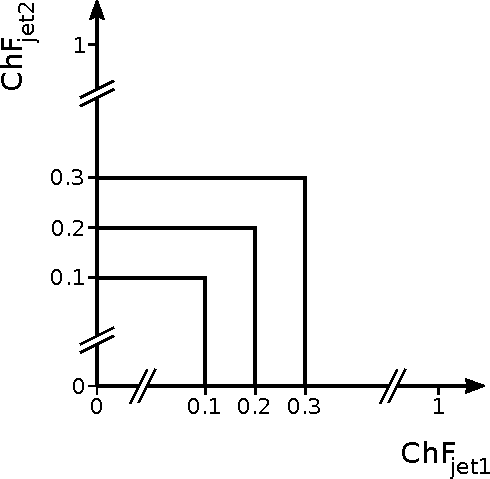
\includegraphics[width=0.5\textwidth]{figures/exclusive_binning.pdf}\hfill%
  \caption{Illustration of the exclusive bins in the leading and subleading jet ChF, used for the closure test and the data vs. prediction comparisons.}
  \label{fig:excl_binning}
\end{figure}

\begin{figure}[h]
  \centering
  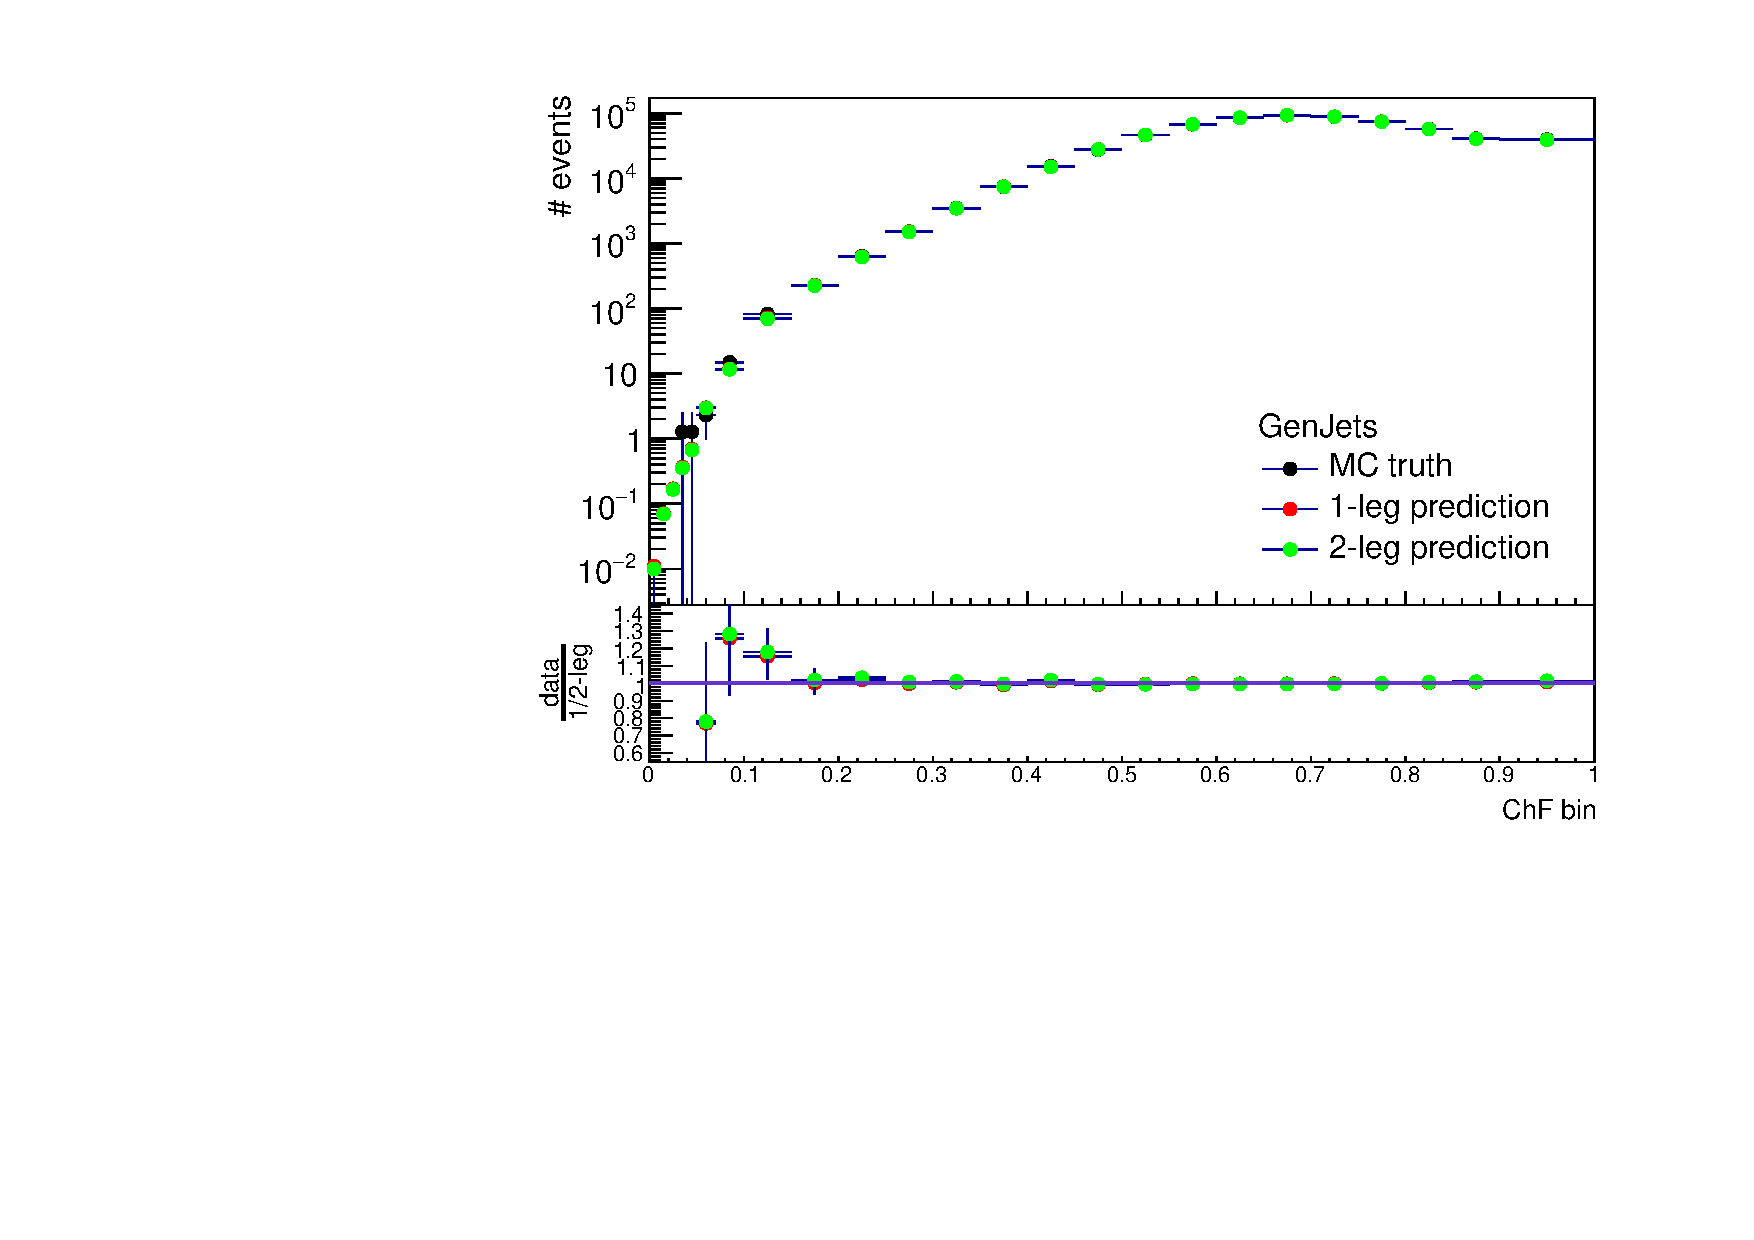
\includegraphics[width=0.75\textwidth]{figures/closure_test_QCD_GenJets_exclusive_correct.pdf}\hfill%
  \caption{Closure test using GenJets.}
  \label{fig:closuretest_GenJets}
\end{figure}

Next, we look at the closure test with reconstructed jets, which is shown in the left plot of Figure~\ref{fig:closuretest}, using the exclusive binning. For the MC truth, the ChF cut is applied on the 2 leading jets of the standard jet collection, as well as the 2 leading jets of the jet collection created when using the second vertex as primary vertex. This extra cut is a part of the signal region event selection described earlier, designed to remove events where the wrong primary vertex was chosen and the charged fraction of the jets is removed by charged hadron subtraction. However, there is still a discrepancy between MC truth and the prediction at the tightest ChF cuts. This is mainly due to a very small number of events where the wrong vertex was chosen, but where the correct one is not the second one.

The closure test on MC is also performed in inclusive bins, as used in the signal region event selection, by applying a cut on the ChF of both jets. This is shown in the right plot of Figure~\ref{fig:closuretest}, with the applied ChF cut on the x-axis. For the MC truth, the statistical uncertainty is determined  per HT-binned QCD sample, using asymmetric vertical bars with correct coverage for event counts with Poisson variates when less than 10 events remain~\cite{PoissonErrorBars}, and the square root of the remaining number of events otherwise. In this way, the statistical uncertainty correctly reflects the contribution of HT bins with few or no events left. The total statistical uncertainty is then calculated by multiplying the uncertainty per HT bin by the corresponding weight for this HT bin, and adding them quadratically. The systematic uncertainty on the background prediction is then defined as the difference between the MC truth and the prediction, unless it is smaller than the statistical uncertainty on the MC truth. In that case, the uncertainty on the MC truth is taken as systematic uncertainty.

\begin{figure}[h!]
  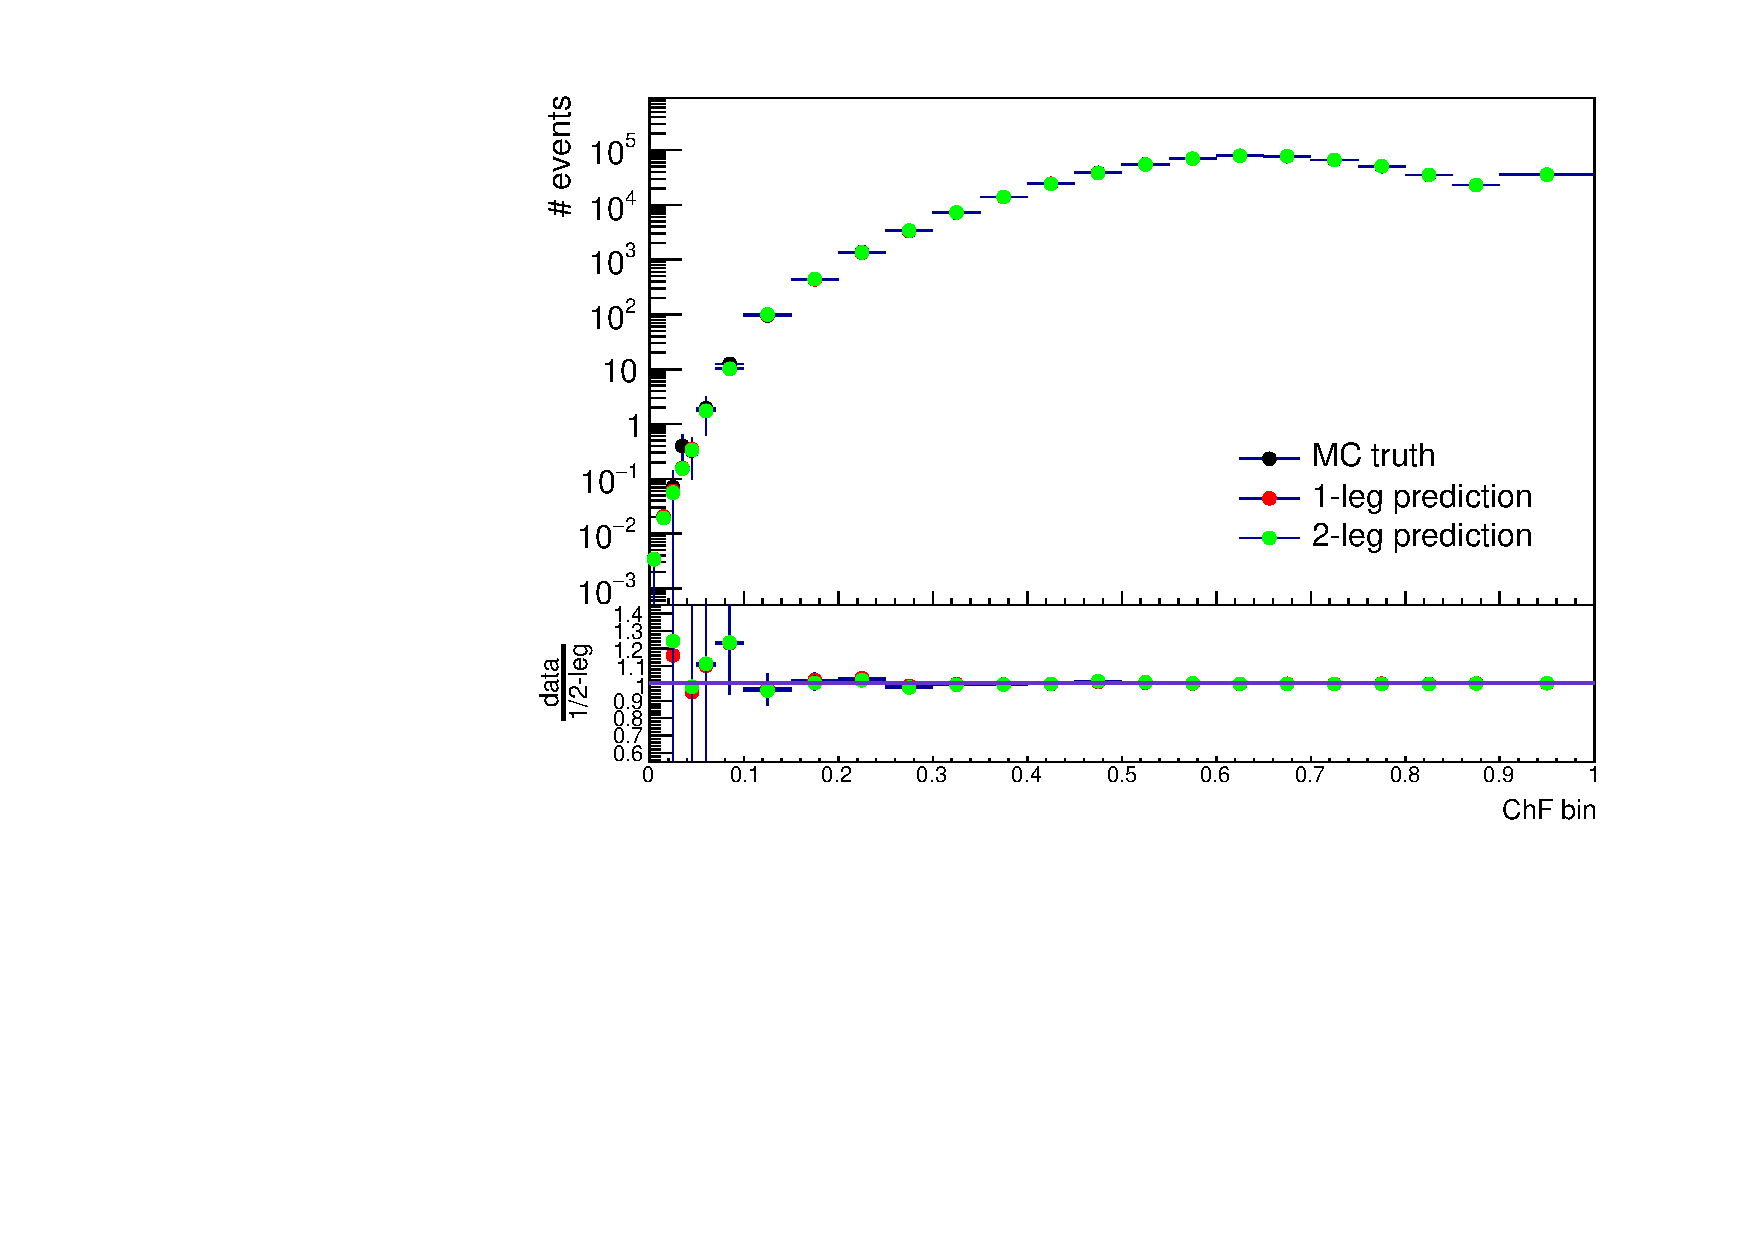
\includegraphics[width=0.5\textwidth]{figures/closure_test_QCD_exclusive_filters.pdf}\hspace{.2cm}%
  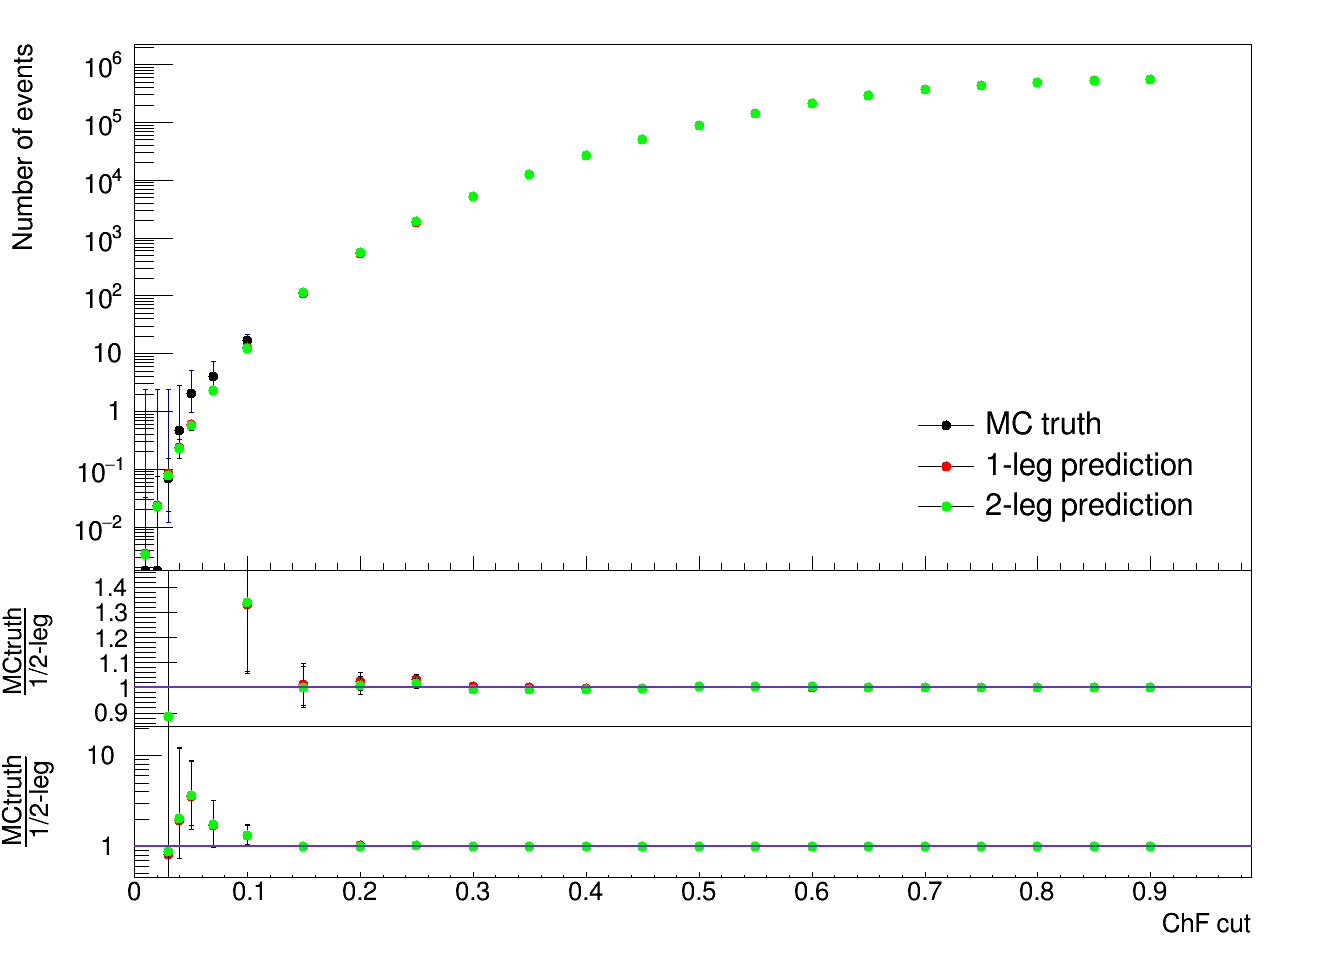
\includegraphics[width=0.45\textwidth]{figures/closure_test_QCD_filters.png}\hfill
  \caption{Closure test in MC using an exclusive (left) or inclusive (right) binning in ChF.}
  \label{fig:closuretest}
\end{figure}

The QCD background prediction in data is shown in Figure~\ref{fig:prediction} as a function of the exclusive ChF bins, using the \texttt{HLT\_PFJet450} single jet trigger. The data is blinded in the signal region below ChF = 0.2. A distinction is made between the run periods B to F (left) and G to H (right). There is a clear deviation below a ChF of 0.4 for run periods B-F, while the agreement is very good down to ChF = 0.2 for G and H. The main difference between these 2 datasets is the issue with the Tracker APV pre-amplifier saturation, which was solved from run period G onwards. The effect of this issue is clearly visible on the number of hits per track, shown in Figure~\ref{fig:nhits} per run period. 

\begin{figure}[h]
  \centering
  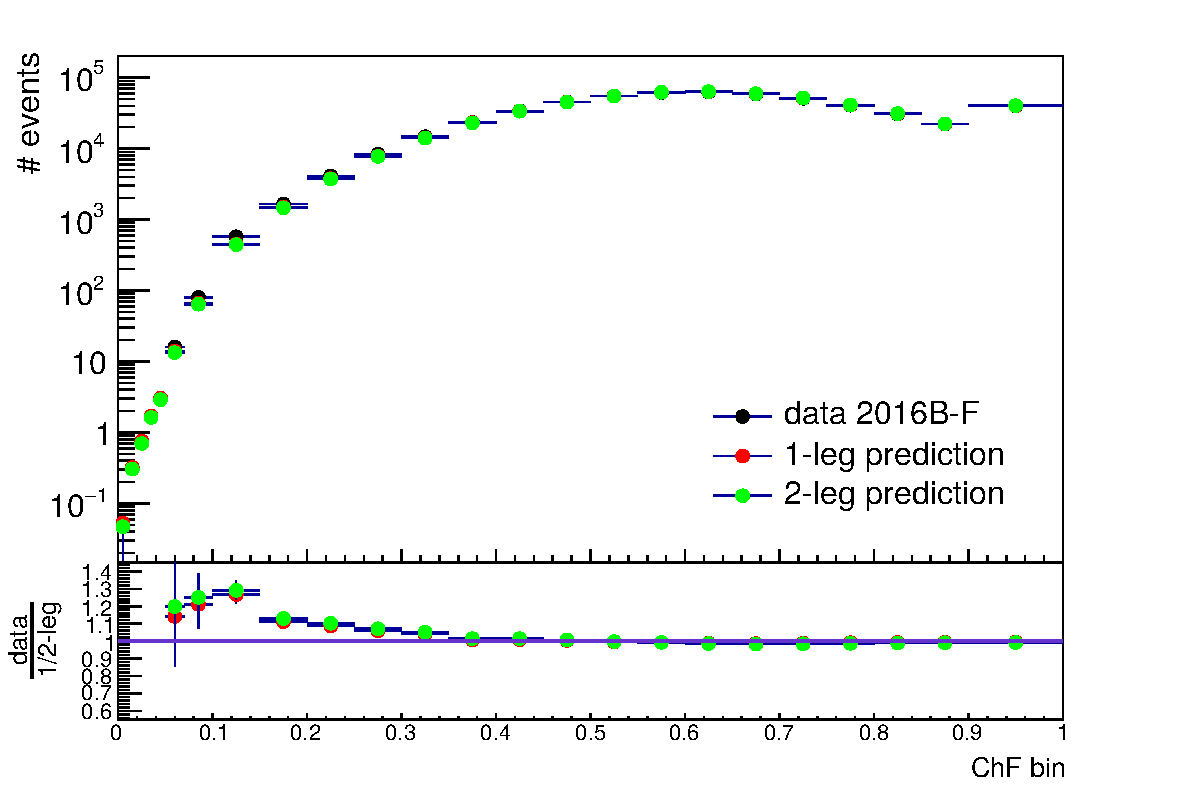
\includegraphics[width=0.5\textwidth]{figures/data_vs_prediction_BF_filters.pdf}\hfill%
  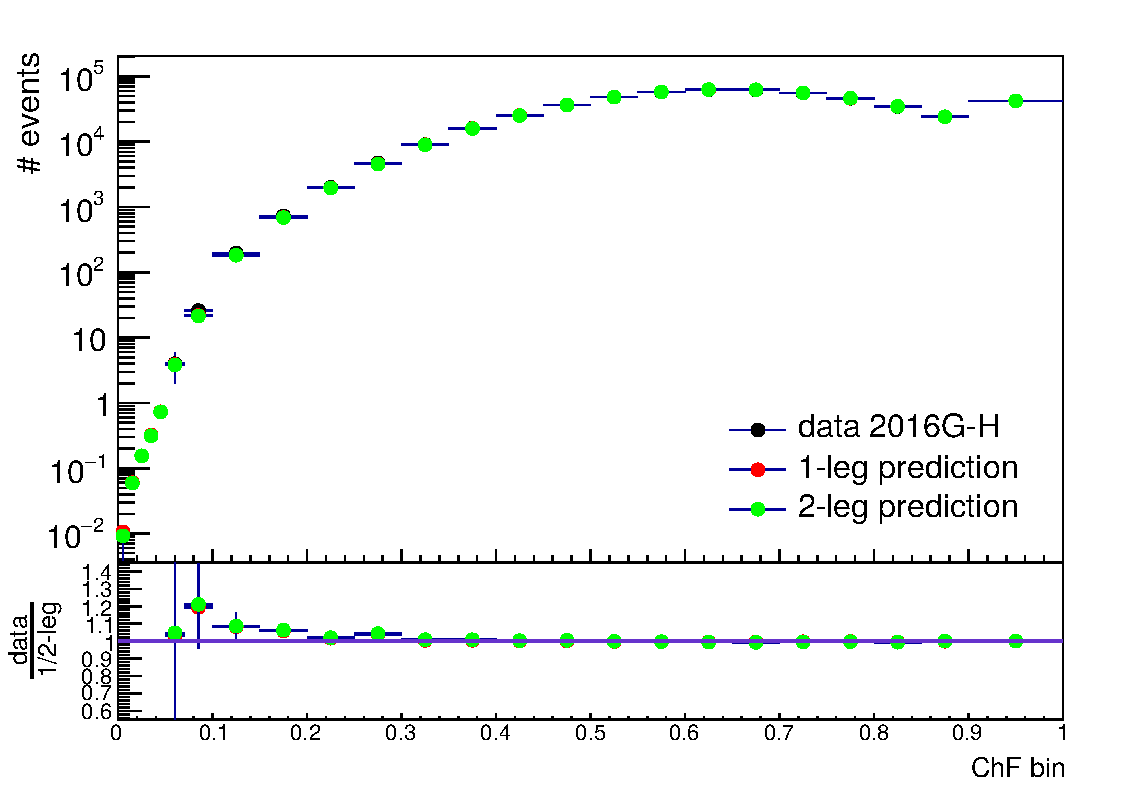
\includegraphics[width=0.5\textwidth]{figures/data_vs_prediction_GH_filters.pdf}
  \caption{The 1- and 2-leg predictions from data, as well as the data (above ChF = 0.2) as a function of the exclusive ChF bins, for run periods B-F (left) and G-H (right).}
  \label{fig:prediction}
\end{figure}

\begin{figure}[h]
  \centering
  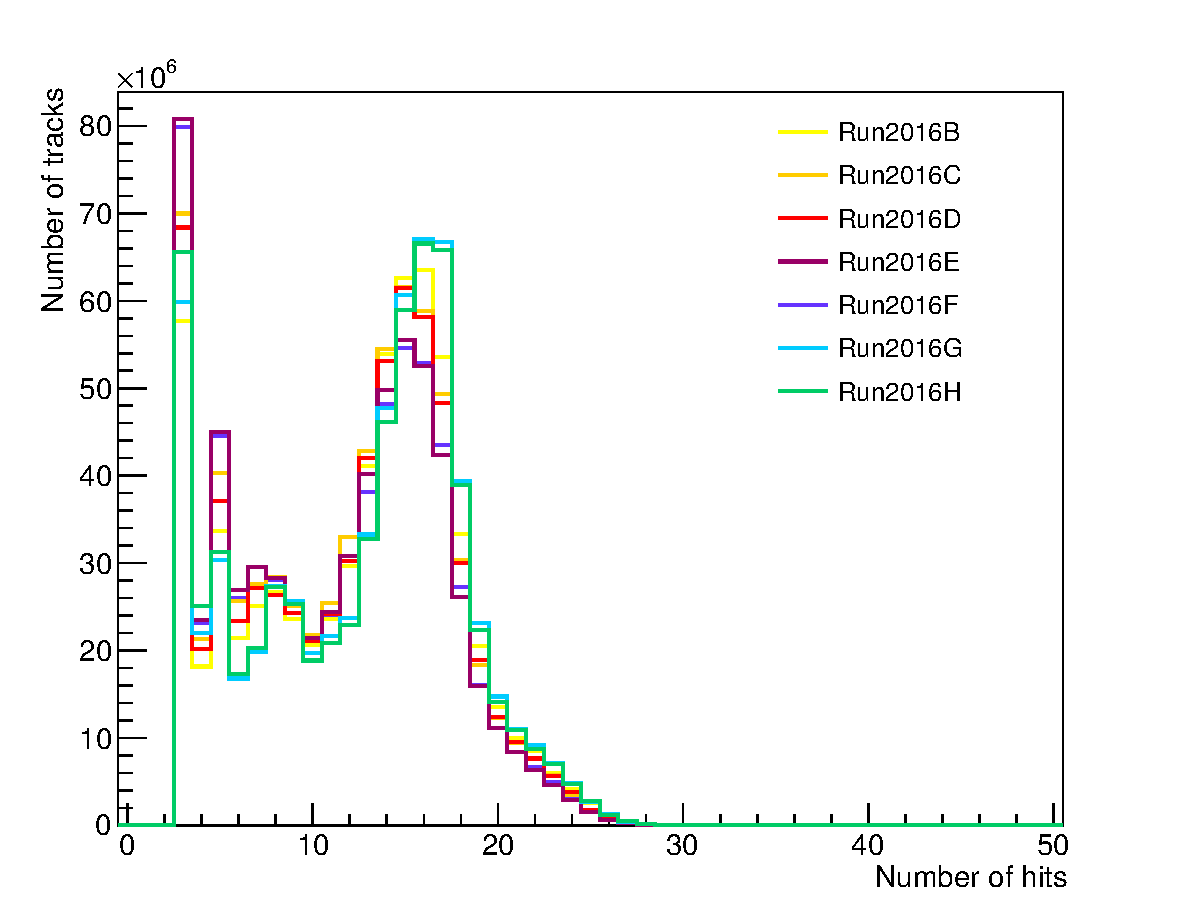
\includegraphics[width=0.8\textwidth]{figures/nhits_perRunPeriod.pdf}\hfill%
  \caption{The number of hits per track, per run period.}
  \label{fig:nhits}
\end{figure}

To first order, the measured ChF cut efficiencies should absorb the effects of tracking inefficiencies caused by the APV pre-amplifier saturation problem. However, this effect is also reflected in the distribution of the number of vertices. As is shown in Figure~\ref{fig:nvtx_reweighting}, a subtle effect causes the data and the prediction from data to disagree in the distribution of the number of vertices for run periods B to F, while a good agreement is obtained for run periods G to H. As we found that there are not enough statistics in order to derive the ChF efficiencies reliably in bins of number of vertices as well as $p_T$ and $\eta$, a recovery of this data in this way is not possible. A reweighting was also performed, using a fit to the ratio of data divided by the 2-leg prediction per ChF bin. Figure~\ref{fig:BF_reweighted} shows the data versus data prediction comparison in run period E, applying the reweighting based on the number of vertices in the event, per ChF bin, and a clear improvement can be observed for the 2-leg prediction. In contrast, the 1-leg prediction has not been reweighted and still shows the original disagreement. This reweighting can however not be used in the signal region, where very few events remain. As a result, the analysis is being performed with run periods G and H only for now.

\begin{figure}[h]
  \centering
  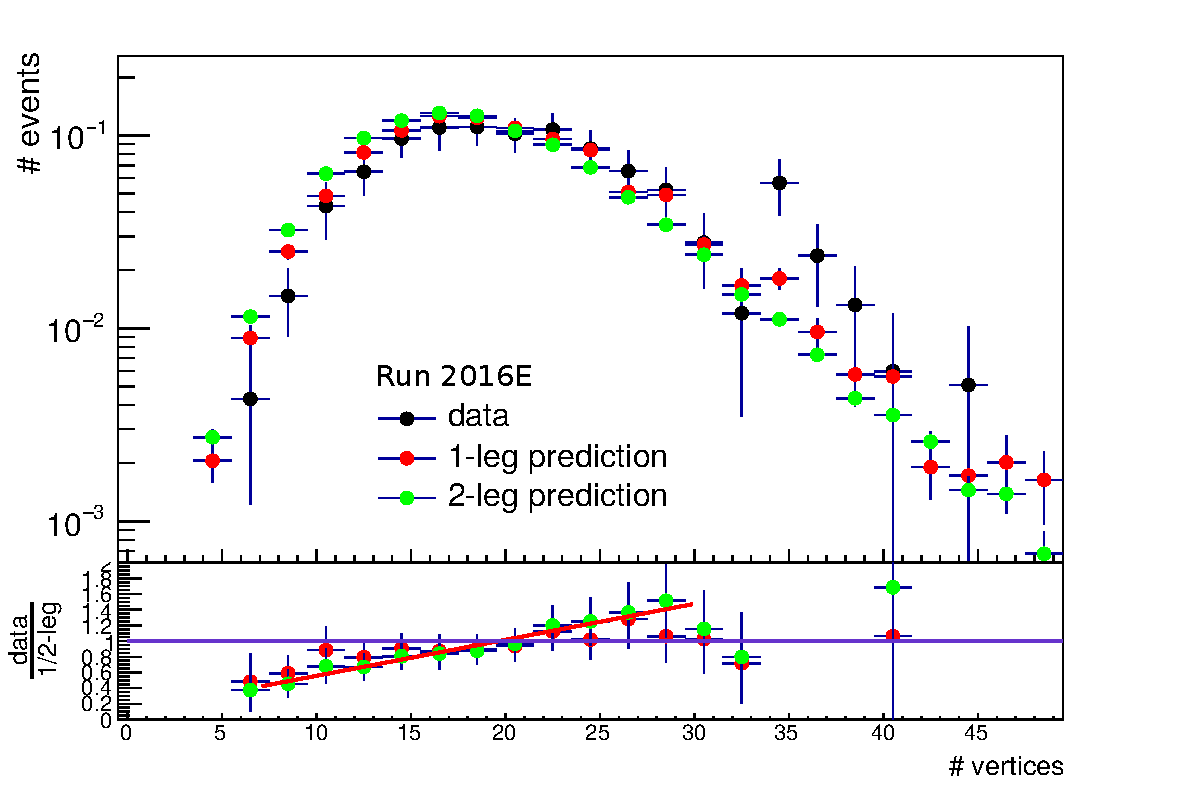
\includegraphics[width=0.5\textwidth]{figures/Data_distributions_excl_RunE_ChF0p25To0p3_nvtx.pdf}\hfill%
  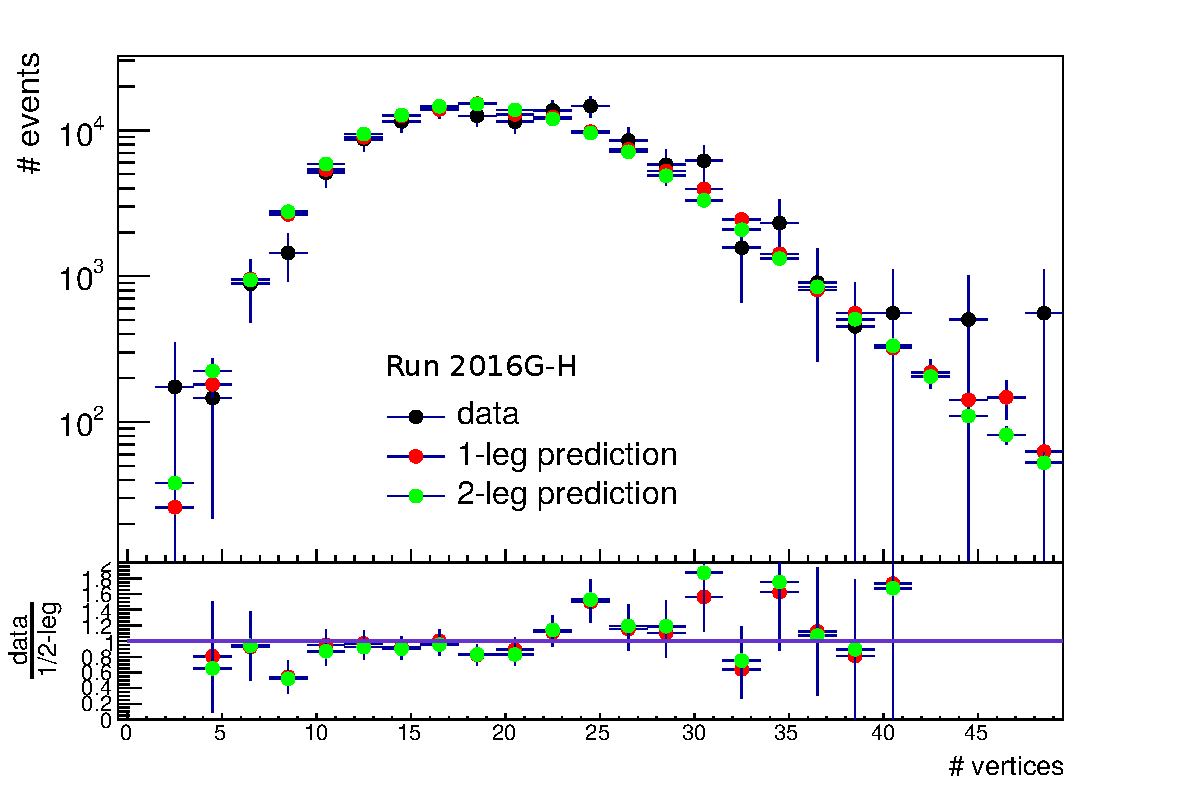
\includegraphics[width=0.5\textwidth]{figures/RunGH_ChF0p25To0p3_nvtx.pdf}
  \caption{The distribution of the number of vertices for data, 1-leg, and 2-leg prediction using data from run period E (left) and run periods G-H (right).}
  \label{fig:nvtx_reweighting}
\end{figure}

\begin{figure}[h]
  \centering
  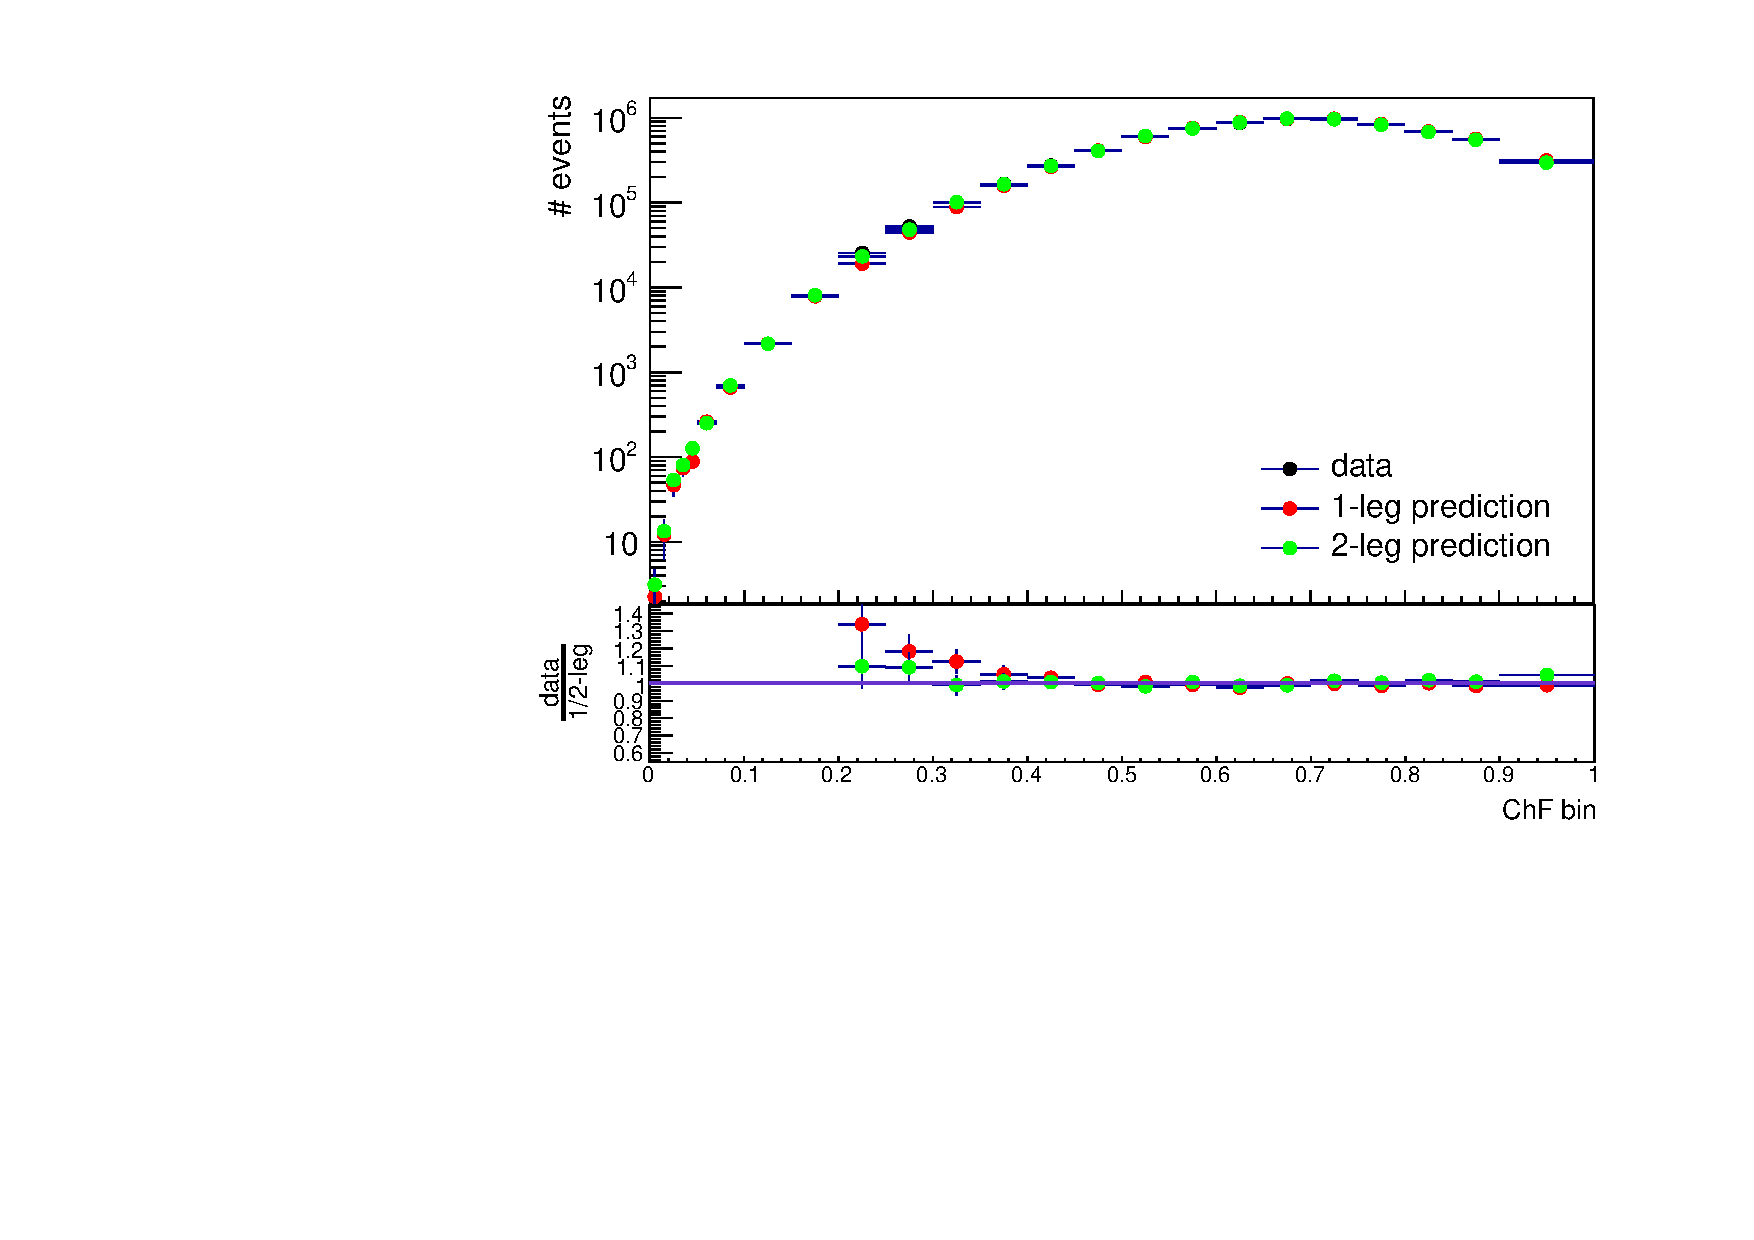
\includegraphics[width=0.7\textwidth]{figures/data_vs_prediction_RunE_reweighted_exclusivebinning.pdf}\hfill%
  \caption{The 1- and 2-leg predictions from data, as well as the data (above ChF = 0.2) as a function of the exclusive ChF bins for run period E, reweighting the 2-leg prediction to data based on the number of vertices in the event, per ChF bin.}
  \label{fig:BF_reweighted}
\end{figure}

\section{Systematic uncertainties}

For the signal prediction, systematics are included for the luminosity, the jet energy corrections, and the trigger inefficiency at 550 GeV due to the turn-on. The systematic for the luminosity amounts to 2.5\%. The systematic uncertainty coming from the jet energy corrections is computed by varying the jet energy by the correction and recalculating the yield after applying the selection cuts and the ChF cut. Depending on the SIMP mass and the ChF cut, this uncertainty varies between 0.4\% and 3.9\%. A systematic uncertainty is also included to take into account the trigger inefficiency at 550 GeV due to the turn-on. This is done by taking a 100\% uncertainty on the efficiency, which gives a 2\% systematic uncertainty for the signal. The photon and conversion veto was found to be 100\% efficient on the signal, and this systematic is therefore found to be negligible. 
%For the cut on the ChF we use 100\% uncertainty by taking the full inefficiency of the cut. This systematic also depends on the SIMP mass and the applied ChF cut and is found to be very small, below 0.5\%. 
The effect of pileup was considered to be negligible, as the distribution of the number of vertices is very similar for the data and SIMP samples. As an example the data is compared to the SIMP sample with $m_{\chi} = 1000$~GeV in Figure~\ref{fig:PU}, which shows there is a good agreement in the bulk of the distribution with some deviations in the tails only.

\begin{figure}[h]
  \centering
  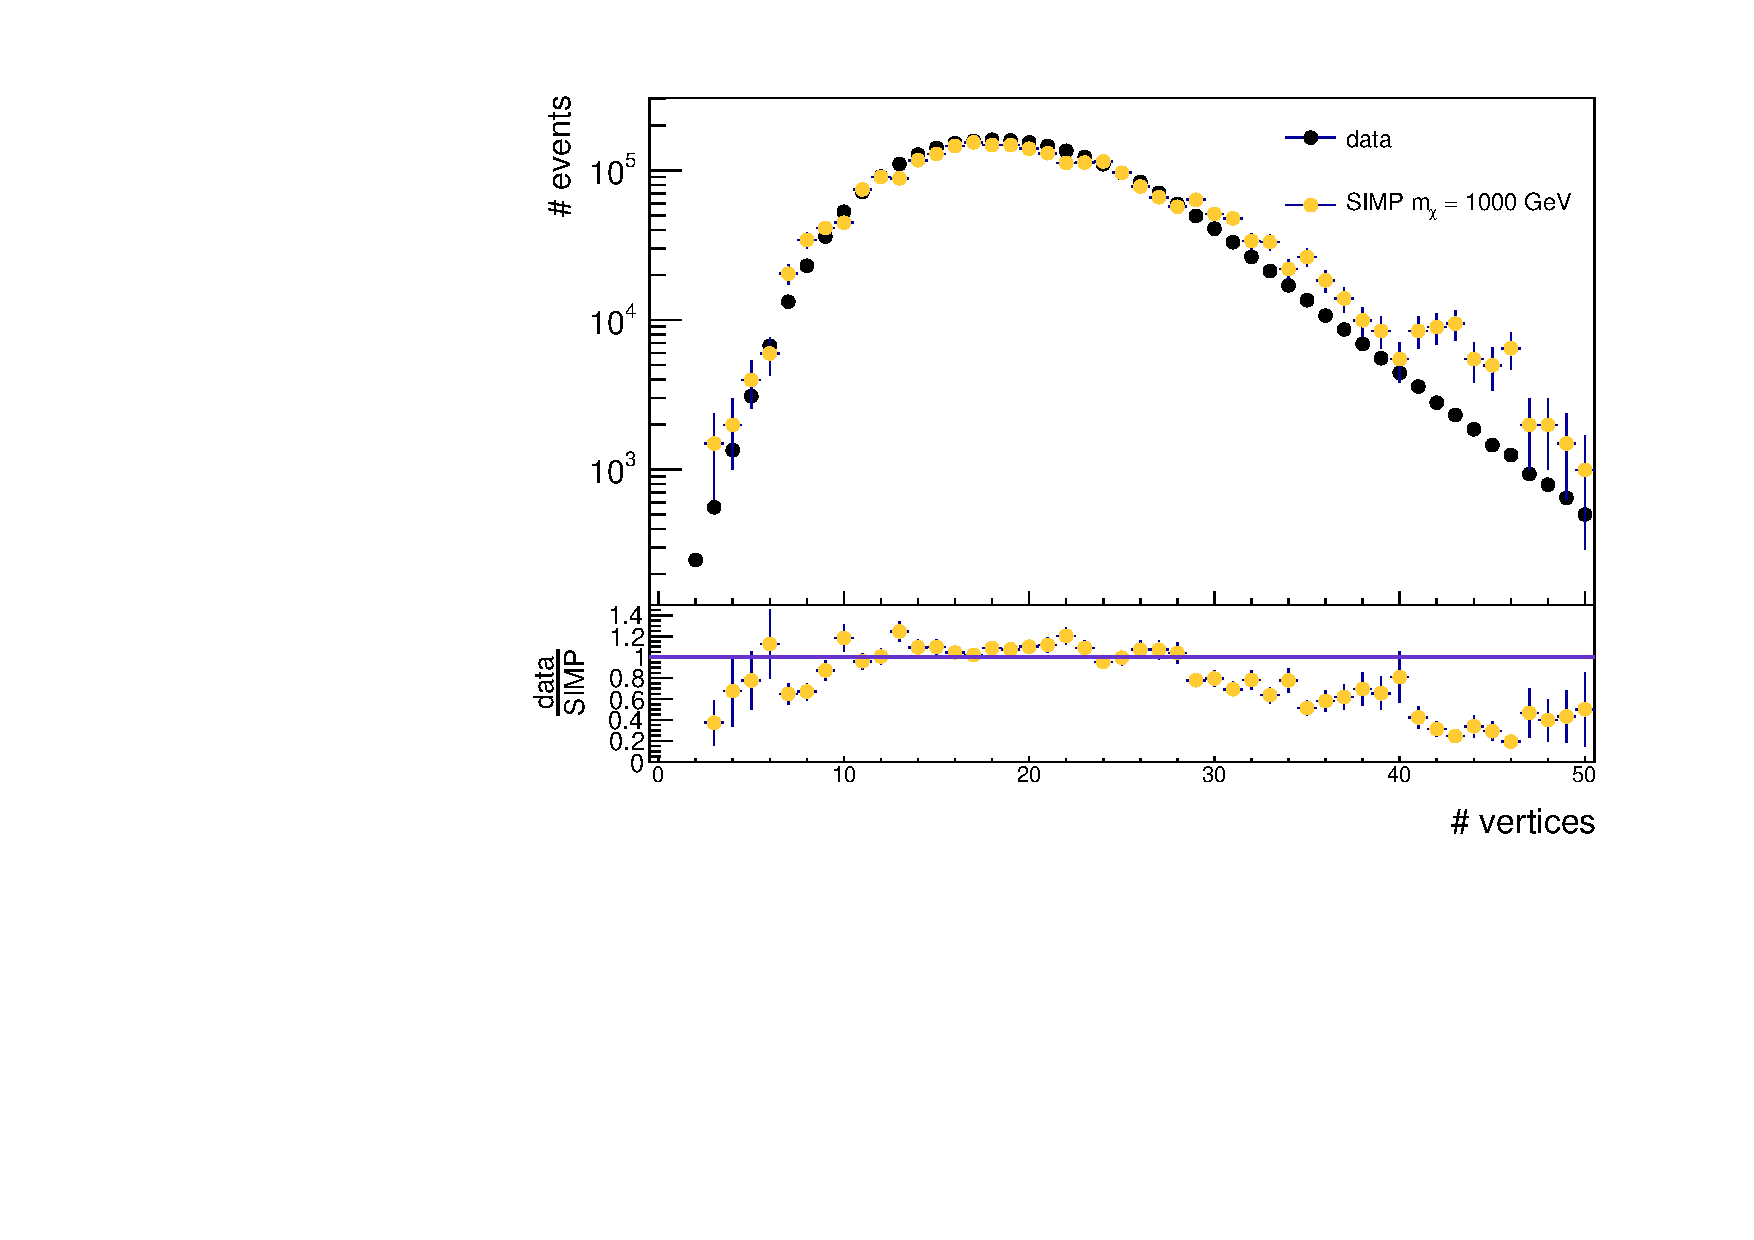
\includegraphics[width=0.7\textwidth]{figures/PU_reweighting_SIMP_M-1000.pdf}\hfill%
  \caption{The distribution of the number of vertices in data compared to the SIMP signal with $m_{\chi} = 1000$~GeV.}
  \label{fig:PU}
\end{figure}

As mentioned in Section~\ref{sec:SIMP_backgrounds}, the main systematic uncertainty on the background prediction is obtained from the closure test in MC, by taking the difference between the MC truth and the prediction, unless it is smaller than the statistical uncertainty on the MC truth, in which case the uncertainty on the MC truth is taken as systematic uncertainty. This uncertainty varies between 4\% and 250\%, depending on the ChF cut. As for the signal, the trigger inefficiency due to the turn-on at 550 GeV is also taken into account.  This yields an additional 2\% systematic uncertainty.

\section{Results}

Table~\ref{tab:results} shows the number of predicted and observed events, per considered ChF cut. The prediction is done using the 1-leg data prediction, as this provides slightly smaller uncertainties. The statistical uncertainty, as well as the systematic uncertainty from the closure test described in Section~\ref{sec:SIMP_systematics}, are given.

We choose a cut of $\mathrm{ChF} < 0.05$ to reject most of the QCD background. The background is then reduced to the level of about one event, and a large uncertainty does not have big consequences. Moreover, the uncertainty from the closure test is reduced when taking into account the smaller statistical uncertainty on the number of background events during the limit calculation. In addition, the expected sensitivity does not improve significantly at tighter ChF cuts, and the closure tests start to run out of statistics. The dominating uncertainty then comes from the closure test, and amounts to 250\% in this case. For the tighter cuts, $\mathrm{ChF} < 0.04$ or $\mathrm{ChF} < 0.03$, the uncertainty from the closure test amounts to 614\% and 3416\%, respectively.

\renewcommand{\arraystretch}{1.3}
\begin{table}[h]
  \centering
\begin{tabular}{| c | r@{$\,\,$}r@{$\,\,$}r@{$\,\,$}r@{$\,\,$}r | r@{$\,\,$}r@{$\,\,$}r | r | r | r |}
\hline
\multirow{2}{*}{ChF cut} & \multicolumn{5}{c|}{\multirow{2}{*}{data prediction}} &  \multicolumn{3}{c|}{QCD MC} & \multirow{2}{*}{observed} & \multicolumn{2}{c |}{SIMP signal [$m_{\chi}$]} \\
\cline{11-12}
 &  &  & & & & \multicolumn{3}{c|}{prediction} & & 1 GeV & 1000 GeV\\
\hline
0.2 & 902 & $\pm$ & 5 (stat.) & $\pm$ & 38 (syst.) & 546.5  & $\pm$ & 0.6 & 969 & 634 & 4.9 \\
0.15 & 210 & $\pm$ & 2 (stat.) & $\pm$ & 18 (syst.) & 111.1  & $\pm$ & 0.4 & 229 & 634 & 4.9 \\
0.1 & 26.9 & $\pm$ & 0.3 (stat.) & $\pm$ & 8.9 (syst.) & 12.6  & $\pm$ & 0.2 & 30 & 634 & 4.9 \\
0.07 & 5.1 & $\pm$ & 0.1 (stat.) & $\pm$ & 4.4 (syst.) & 2.3  & $\pm$ & 0.2 & 4 & 634 & 4.9 \\
0.05 & 1.28 & $\pm$ & 0.03 (stat.) & \multicolumn{2}{l |}{$\!\!\!^{+\ 3.24}_{-\ 1.28\,}$ (syst.)} & 0.6  & $\pm$ & 0.1 & 0 & 634 & 4.9 \\
0.04 & 0.55 & $\pm$ & 0.02 (stat.) & \multicolumn{2}{l |}{$\!\!\!^{+\ 2.81}_{-\ 0.55\,}$ (syst.)} & 0.24  & $\pm$ & 0.09 & 0 & 633 & 4.9 \\
0.03 & 0.22 & $\pm$ & 0.01 (stat.)& \multicolumn{2}{l |}{$\!\!\!^{+\ 7.68}_{-\ 0.22\,}$ (syst.)} & 0.08  & $\pm$ & 0.07 & 0 & 632 & 4.9 \\
\hline
\end{tabular}
\caption{Number of predicted (using the 1-leg prediction from data) and observed events for the considered cuts. The expected number of signal events is also given for the $m_{\chi} = 1$ GeV and $m_{\chi} = 1000$~GeV scenarios.}
\label{tab:results}
\end{table}

We calculate the model-independent limits for a ChF $<$ 0.05 cut, using the $CL_S$ criterion~\cite{CLS1,CLS2} with the LHC style test statistic in which the systematic uncertainties are modeled as nuisance parameters. This was done using the RooStat-based Combine tool~\cite{combine}, taking into account the  systematic uncertainties detailed in Section~\ref{sec:SIMP_systematics}, as well as the statistical uncertainties on signal and background predictions. All included systematic uncertainties are profiled with a lognormal prior, except for the uncertainty coming from the closure test, which is profiled with a gamma function since it comes from limited statistics. The resulting expected fiducial cross section is $\sigma_{\mathrm{fid}}^{95\%} = \sigma\times\mathrm{A}\times\epsilon = 0.17$~fb. With zero observed events, the observed model-independent limit is found to be $\sigma_{\mathrm{fid, obs}}^{95\%} = 0.18$~fb.

\section{SIMP model interpretation}

Limits were also derived on the production cross section for the SIMP model with the considered mass points, using the same method as described for the model-independent limits.  The expected limits on the production cross section are shown for SIMP masses between 1 and 1000~GeV in Figure~\ref{fig:SIMP_limit}, using a cut of $\mathrm{ChF} < 0.05$. In this case, the search is sensitive to all the generated SIMP mass points, up to 1000~GeV. For completeness, the obtained expected limits in the case of a ChF cut at 0.03 or 0.04 can be found in Appendix~\ref{sec:app_limits}.

Figure~\ref{fig:SIMP_limit_unblinded} shows the expected and observed limits after unblinding. The expected and observed limits, and the theoretical cross section are given with respect to the generator level cuts applied in the signal sample generation, $p_T^{\chi} > 200$~GeV and $|\eta_{\chi}| < 2.5$. The shown theoretical cross section is also given per SIMP mass point in Table~\ref{tab:signal_samples}.

\begin{figure}[h]
  \centering
  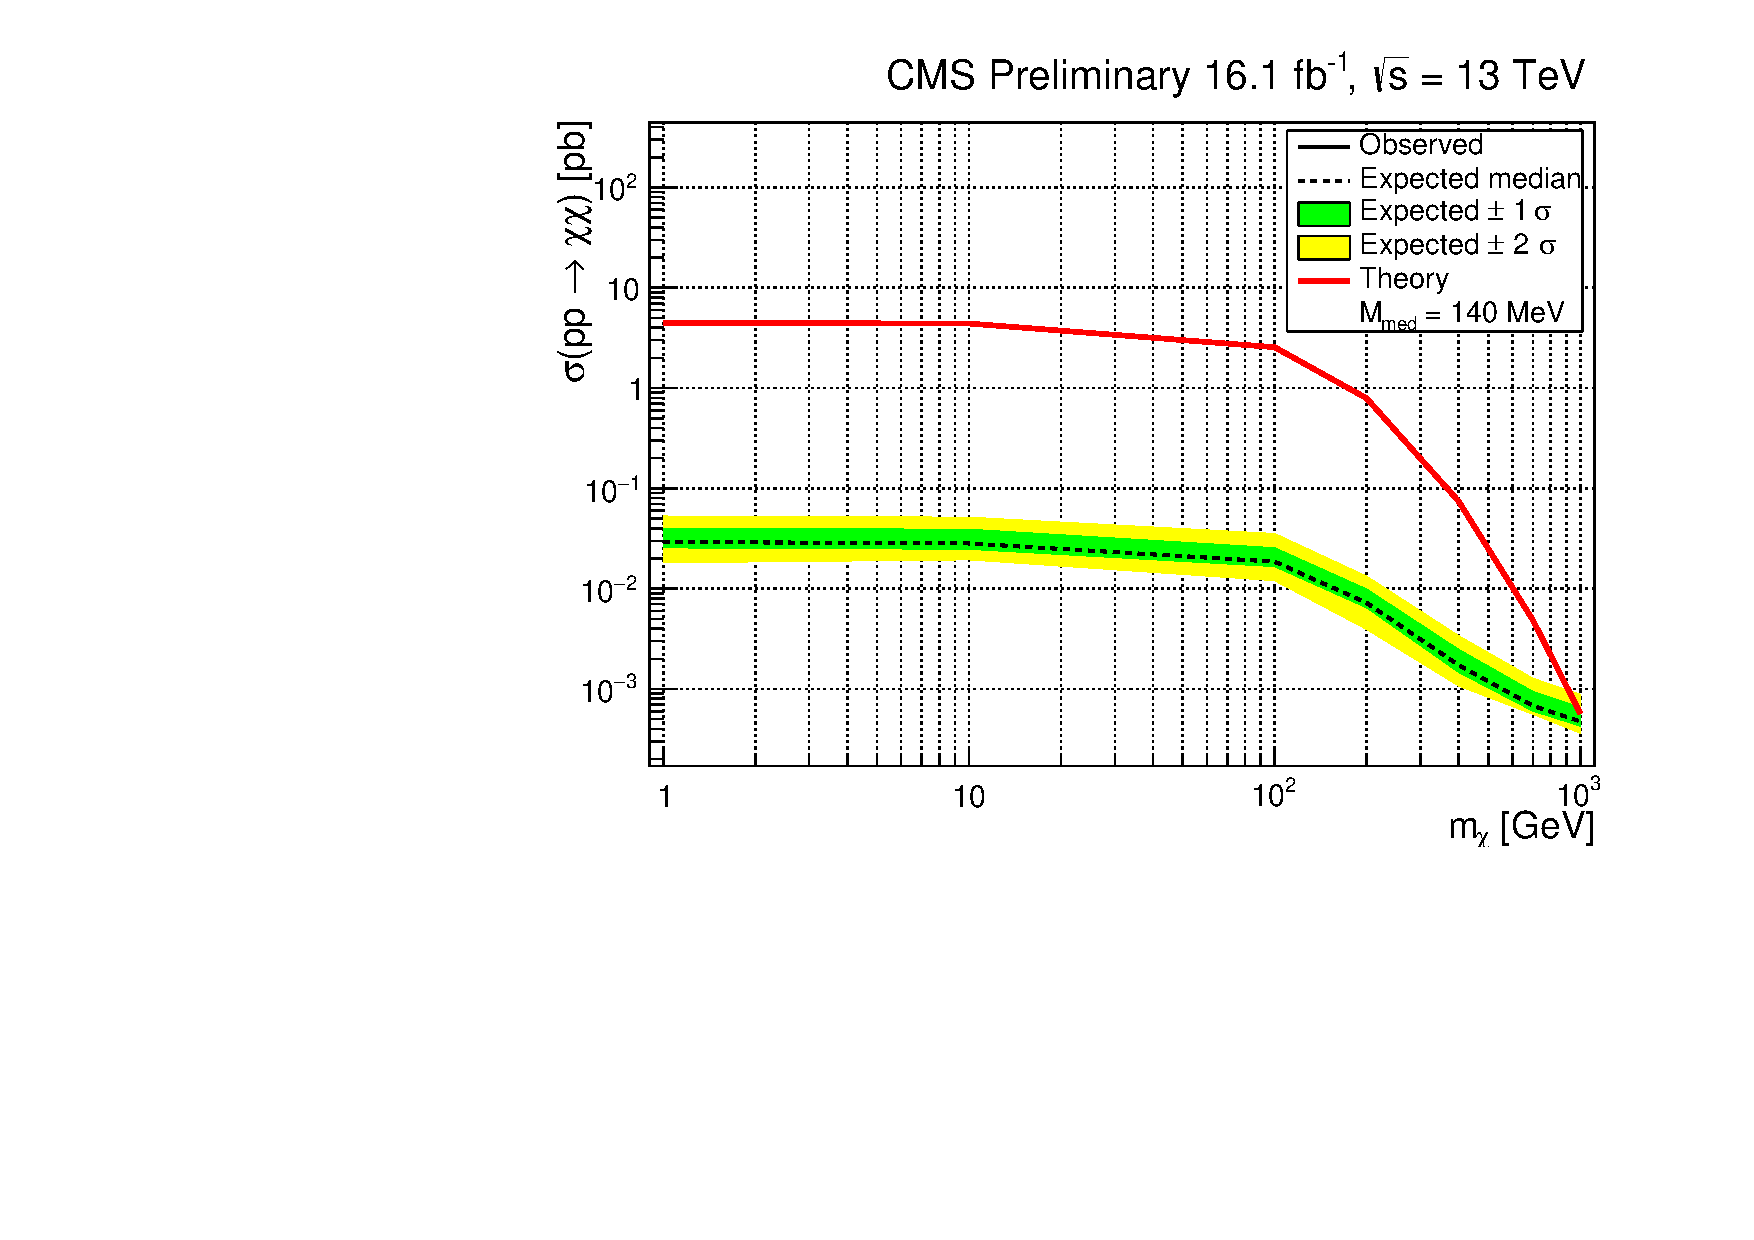
\includegraphics[width=0.8\textwidth]{figures/SIMP_limit_ChF0p05.pdf}\hfill%
  \caption{The expected limits on the production cross section, obtained without looking in the signal region, for SIMP masses between 1 and 1000~GeV, with $1\sigma$ and $2\sigma$ bands is shown, as well as the theoretical prediction (red), with respect to the generator level cuts ($p_T^{\chi} > 200$~GeV and $|\eta_{\chi}| < 2.5$).}
  \label{fig:SIMP_limit}
\end{figure}

\begin{figure}[h]
  \centering
  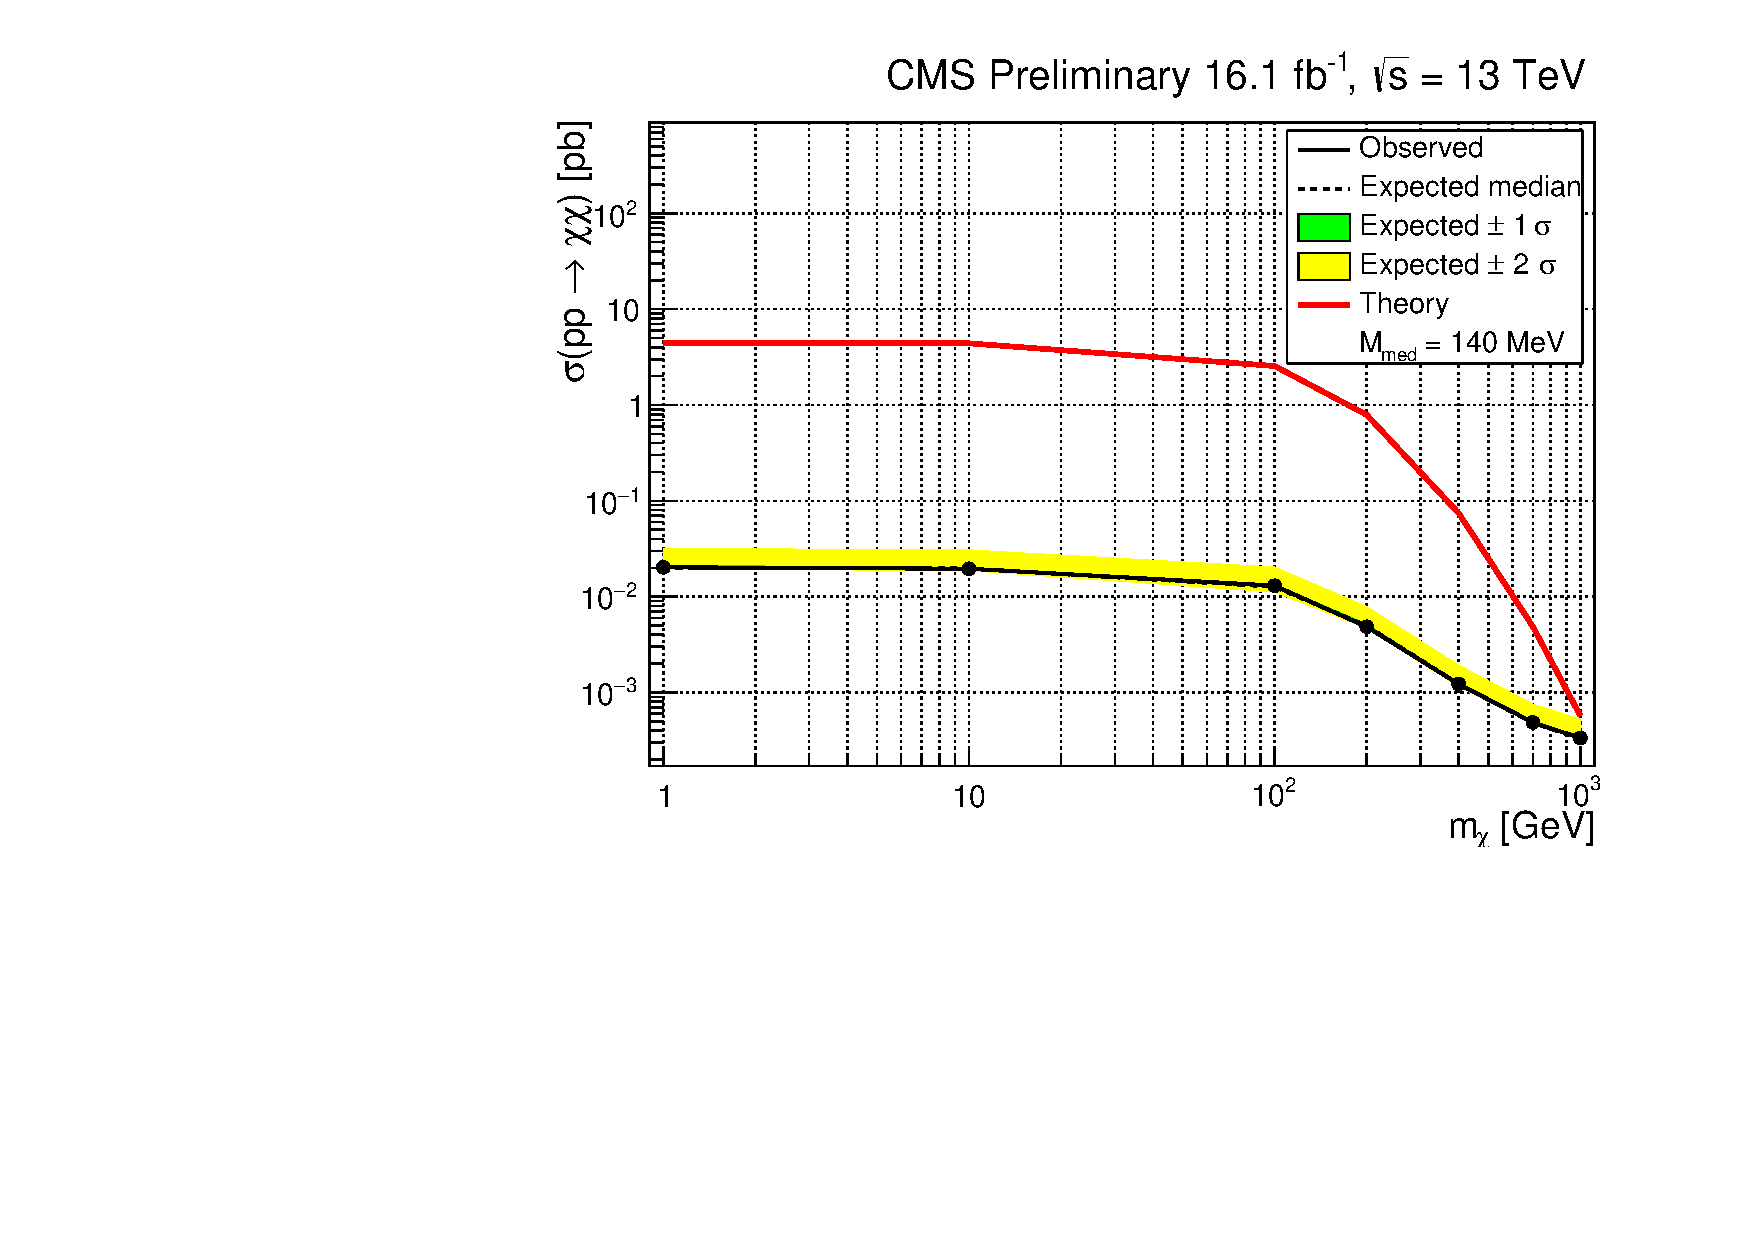
\includegraphics[width=0.8\textwidth]{figures/SIMP_limit_ChF0p05_unblinded.pdf}\hfill%
  \caption{The expected and observed limits on the production cross section for SIMP masses between 1 and 1000~GeV, with $1\sigma$ and $2\sigma$ bands is shown, as well as the theoretical prediction (red), with respect to the generator level cuts ($p_T^{\chi} > 200$~GeV and $|\eta_{\chi}| < 2.5$).}
  \label{fig:SIMP_limit_unblinded}
\end{figure}

\clearpage


\clearpage{\pagestyle{empty}\cleardoublepage}
